\documentclass{report}
\usepackage{textcomp}
\usepackage{mathtools}
\usepackage{enumitem}
\usepackage{cite}
\usepackage{titlesec}
\usepackage{graphicx}
\usepackage{float}
\usepackage{hyperref}
\usepackage[section]{placeins}
\usepackage[toc,page]{appendix}
\usepackage[margin=1in]{geometry}
\usepackage[doublespacing]{setspace}
\usepackage[font=scriptsize]{caption}



\graphicspath{ {images/} }
\widowpenalty=1500
\clubpenalty=1500

\titlespacing*{\chapter}{0pt}{0pt}{20pt}
\titleformat{\chapter}[display] {\normalfont\bfseries}{}{0pt}{\centering \LARGE}

\begin{document}
	\begin{titlepage} \begin{singlespace}
        \begin{center} \begin{large}
            UNIVERSITY of CALIFORNIA \\ SANTA CRUZ

            \vspace{\baselineskip}

            \textbf{Adventures in Firing a 30-Year-Old Metal-Cutting Laser \\ at Extremely Sensitive Electronic Circuits \\ and Trying to Not Break Anything}

            \vspace{\baselineskip}

            A thesis submitted in the hope that \\ any future researchers on this project

            \vspace{\baselineskip}

            DO NOT MAKE THE SAME MISTAKES THAT I DID

            \vspace{\baselineskip}

            and

            \vspace{\baselineskip}

            ARE ABLE TO PRODUCE GOOD RESULTS

            \vspace{\baselineskip}

            by

            \vspace{\baselineskip}

            \textbf{Christopher D. Milke}

            \vspace{\baselineskip}

            \today

            \vspace*{\fill}

            \end{large}
        \end{center}

	\end{singlespace} \end{titlepage}


    %copyright
    \newpage \begin{center} \pagenumbering{roman}
        \vspace*{\fill}
        Copyright \textcopyright by

        Christopher D. Milke 

        2016
        \vspace*{\fill}
    \end{center} \newpage


    %abstract
    \addcontentsline{toc}{chapter}{Abstract}
        \begin{center} \LARGE \textbf{Abstract} \end{center}
        I have been attempting to perform laser injection experiments on prototype strip sensors to test the effectiveness of the Punch Through Protection structure. I have performed the experiment with a variety of methods, but each method results in either the tested sensors being destroyed, or the results from the test being unuseable. Using NENIR filters which allow more than 3\% transmission of the laser light invariably result in sensor failure when the sensor is biased near its depletion voltage. However, using NENIR filters with tranmission less than 1\% produce non-sensical results with vast standard deviations in the data points. The use of tissue paper as a means of diffusing laser light produces more extreme versions of the low transmission neutral density filters, with data points that are nearly randomly distributed. Peltier cooling seems to be the only potentially viable method I attempted, with cooling to 0 $^\circ$C and an NENIR 510B or 513B neutral density filter, being a possible way to test PTP equipped sensors safely.



    \newpage


    \tableofcontents


    %dedication and acknowledgments
    \newpage \vspace*{\fill}
        \addcontentsline{toc}{chapter}{Dedication}
        \begin{center} \begin{large}
            Dedicated to all of the brave sensors\\
            who gave their lives in the name of science.
        \end{large} \end{center}
    \vspace*{\fill} \newpage \vspace*{\fill}
        \addcontentsline{toc}{chapter}{Acknowledgements}
        \begin{center} \begin{large}
            \large \textbf{Acknowledgements} \vspace{\baselineskip}

            I would like to give a big thanks to Vitaliy Fadeyev and Zachary Galloway, both of whom were immensly helpful in providing advice, guidance, and technical support during my time doing research at SCIPP. Without their help, I would not have been able to perform, or even think of, anywhere near as many experiments as I did.

        \end{large} \end{center}
    \vspace*{\fill} \newpage





    \pagenumbering{arabic} \setcounter{page}{1}
    \chapter{ Background }
        Sometime after the year 2022, the Large Hadron Collider (LHC) is planned to undergo a massive upgrade to its particle beam. This upgrade, called the High Luminosity LHC, or HL-LHC for short, will ramp the beam luminosity up tenfold, providing a variety of exciting new experimental possibilities, but also presenting a number of potential problems for the sensitive detection equipment surrounding the particle beam. This report focusses on a protype sensor technology that could help to mitigate one of these problems. More specifically, this report focusses on how to perform experiments on and test this prototype technology, or rather, how \textit{not} to test it. Now, what are we testing, and why?
            
        One of the two biggest detectors around the LHC is the ATLAS detector, and in the middle of ATLAS is the Vertex Tracker subsystem. The Vertex Tracker is placed very close to the LHC's beam line, and as such is particularly vulnarable to an incident known as beam misalignment. Ideally, the beams of the LHC will always go straight down their respective beampipes, and all that will hit the Vertex Tracker is the myriads of scattered particles resulting from the beam collisions. If a beam becomes misaligned though, it can shoot directly into the Vertex Tracker, damaging not only the sensors, but also sending dangerously high currents through to the sensitive (and very expensive) readout equipment attached to the sensors. As such, a special type of sensors are in developement to protect the readout electronics. What makes these sensors special is the Punch Through Protection (PTP) structure. The idea is that, if extremely high voltages pass across through a strip on a PTP equipped sensor, then this PTP structure will activate, redirecting the charge on the strip to ground, instead of to the readout electronics. I should add that the term "activate", and in fact even the term "structure" are perhaps a bit advanced for what the PTP structure is and does. In reality, it is no more than the gap between the sensor strip and the bias ring. PTP sensors have a much smaller gap than most sensors, so if the voltage on a strip is too high, it is able to simply jump this gap, shorting the sensor. This sensor shorting between strip and bias ring is the "activation" of the PTP structure. For a much detailed description of PTP structures, see Colin Parker's Bachleour's Thesis (\cite{parker_thesis}) and Christopher Betancourt's Master's Thesis (\cite{betancourt_thesis}).

        What I have been doing for the past year is trying to test the effectiveness of the PTP structure in a variety of sensors. We simulate a beam misalignment by shooting the sensor with an infared laser, a process we call laser injection testing. The current that would be output to the readout electronics is picked up on the strip's dc pads, showing how much of the current was redirected through the PTP structure to the bias ring, and thus how effective the PTP structure is. For more details on the experiment and on the PTP structure itself, I would recommend reading Collin Parkers undergraduate thesis and Chris Betancourt's master thesis. Unfortunately, there will be no discussion of PTP effectiveness in the remainder of this paper. I said I spent the past year \textit{trying} to test PTP effectiveness; I have not succeeded in this endevour. Every single PTP equipped sensor I have ever tested has, without fail, broken during laser injection testing, before any meaningful results could be obtained. This report is a chronology of my various attempts at performing laser injection testing, in the hope that those who perform this test in the future can learn from my mistakes and obtain meaningful results. 





    \chapter{ Laser Injection Testing Setup } \label{sect:methods}
        %setup circuit, put in laser filter
        \section{ Preperation }
            %oscilloscope setup
            The first step to performing laser injection analysis is to turn on the Tektronix TDS 5054 Oscilloscope, as it takes a while to boot up. Once it is on and the oscilloscope screen is visible, make sure the settings are sane. The oscilloscope hardware settings are visible in figure \ref{fig:oscilloscope_01}, with a clearer view of the screen settings in figure \ref{fig:oscilloscope_00}.

            \begin{figure}[h] 
                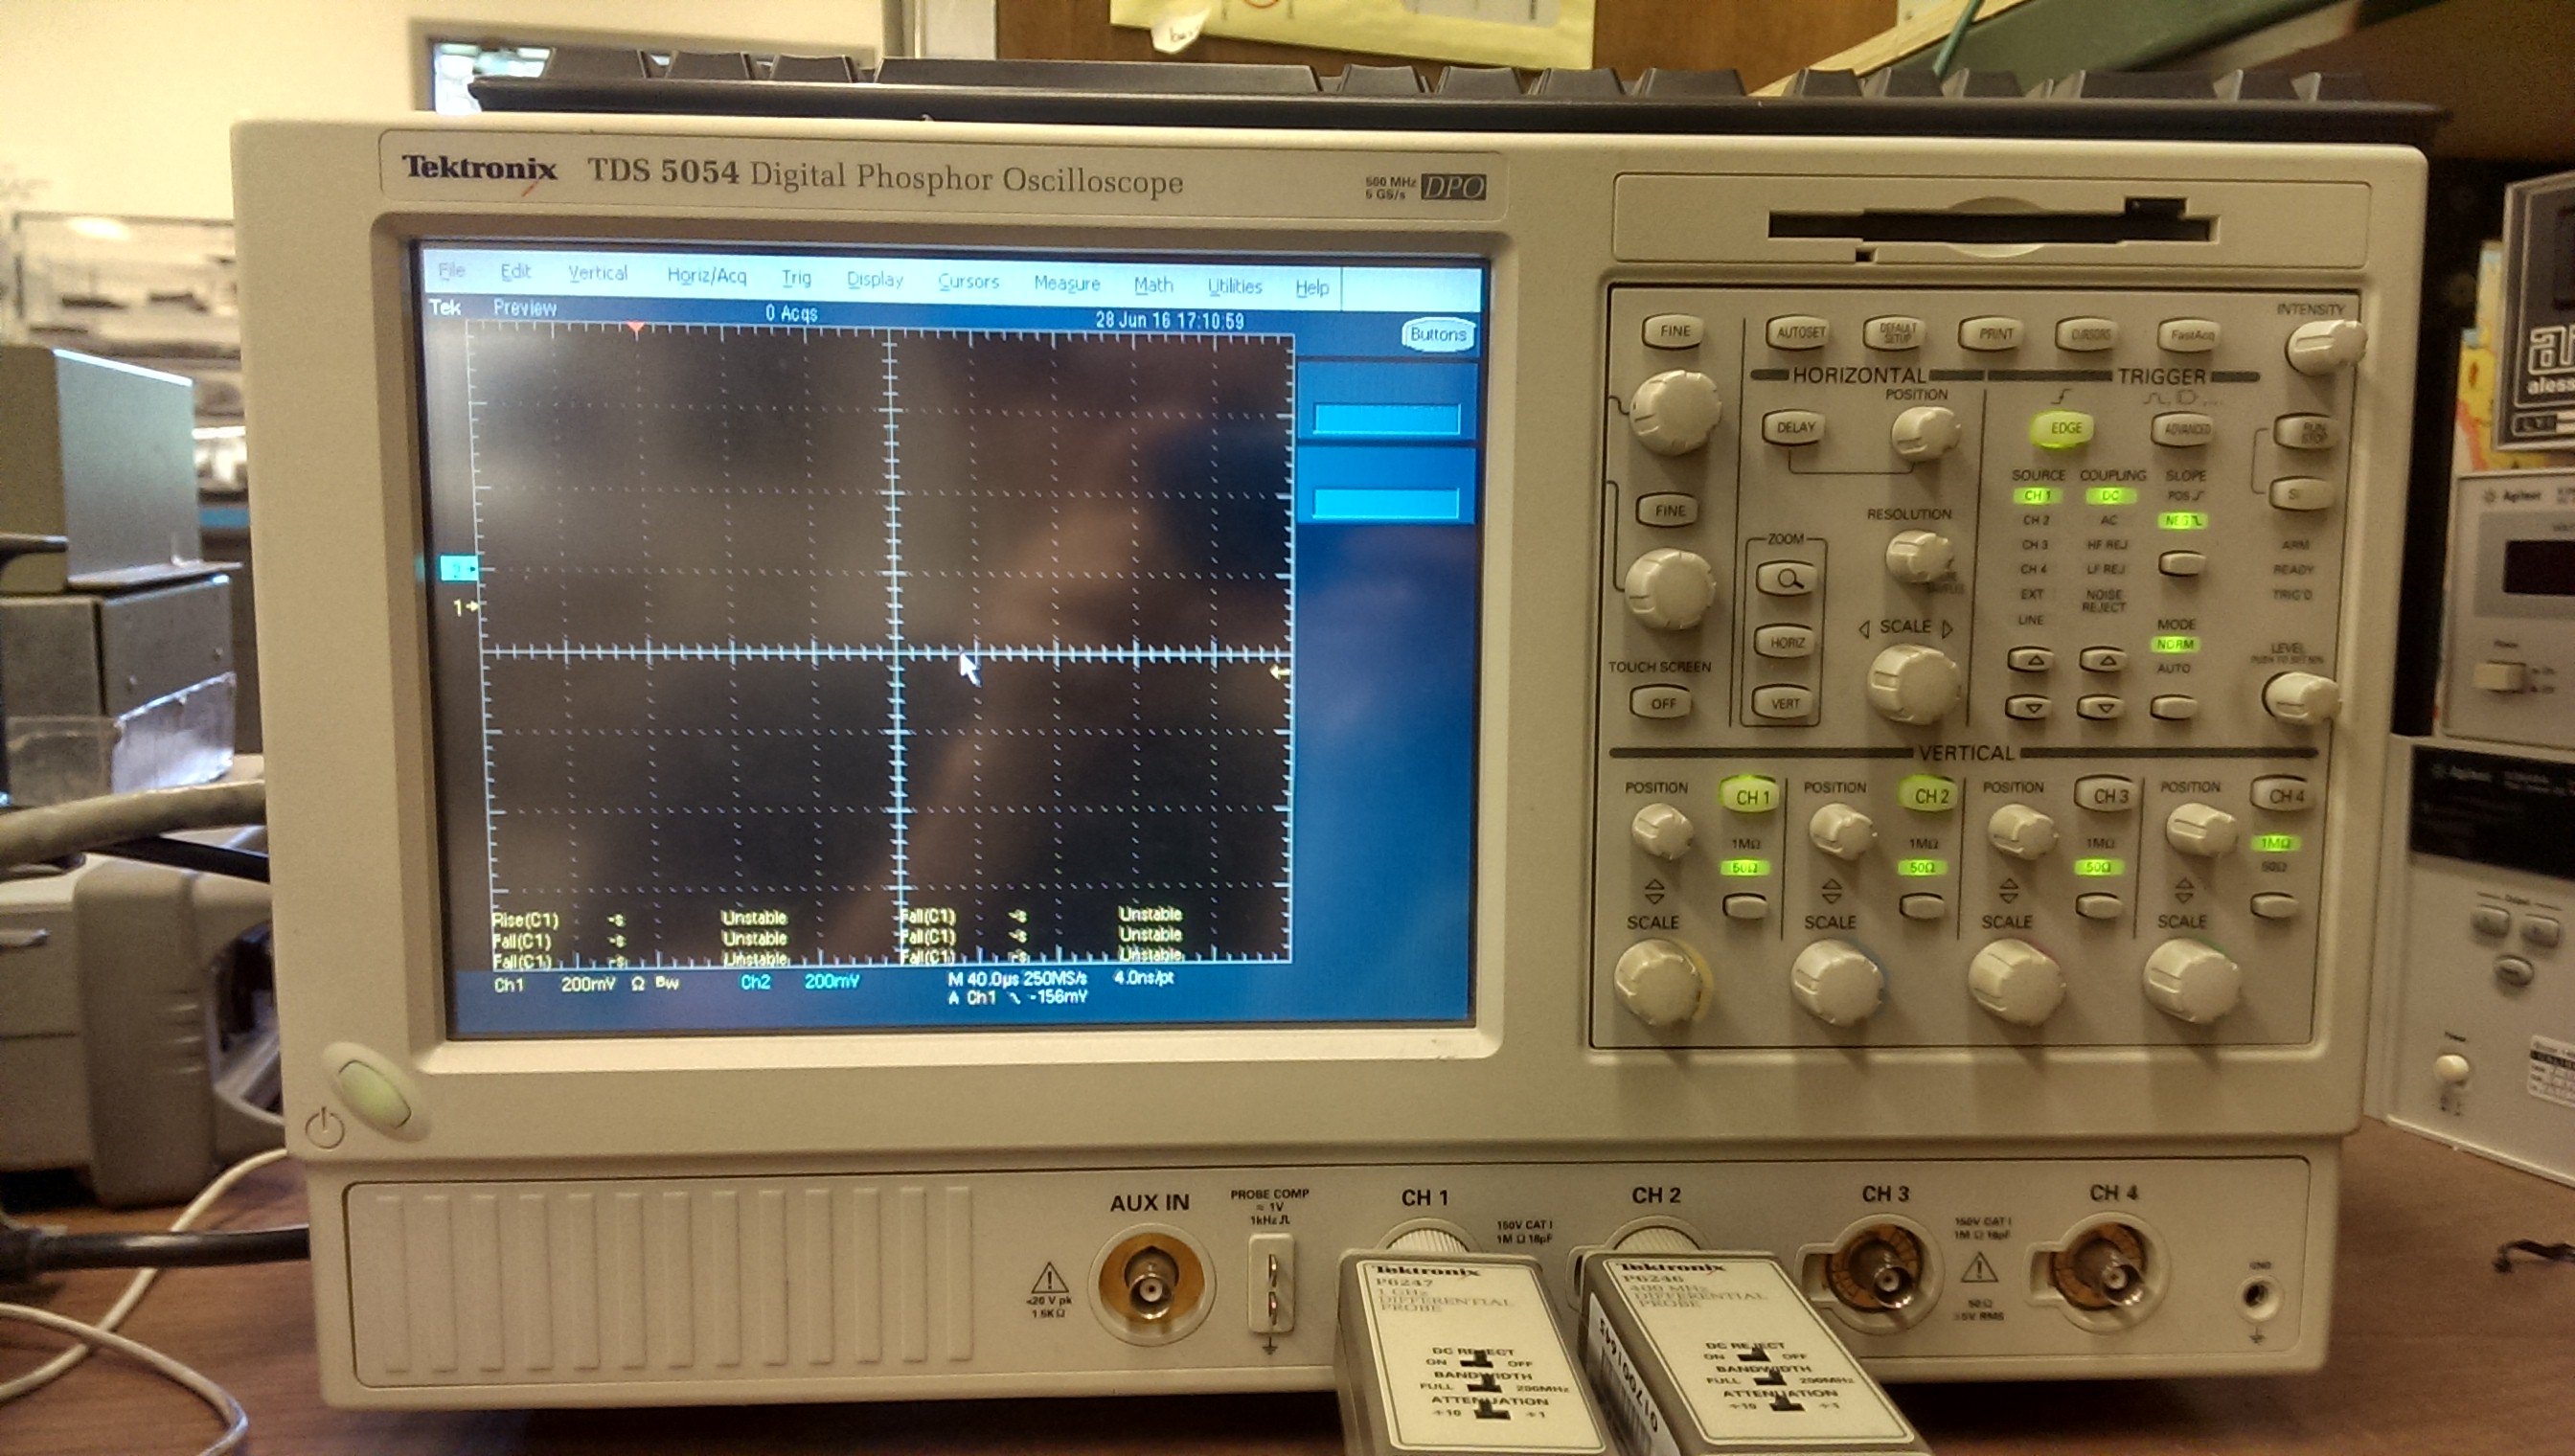
\includegraphics[height=.4\textheight]{oscilloscope_01}
                \centering
                \caption{ A view of the Textronix Oscilloscope, with everything set to operate for laser injection testing.}
                \label{fig:oscilloscope_01}
            \end{figure}

            \begin{figure}[h] 
                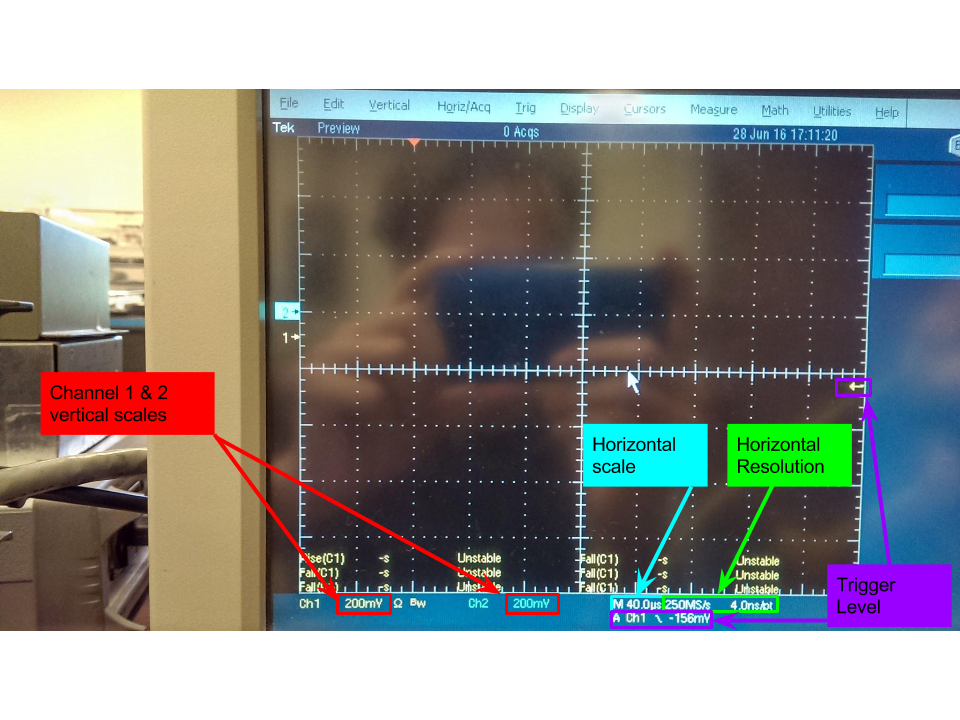
\includegraphics[height=.4\textheight]{oscilloscope_00}
                \centering
                \caption{ A view of the Textronix Oscilloscope viewing window, pointing out the various viewing and resolution settings that I have typically used. }
                \label{fig:oscilloscope_00}
            \end{figure}


            %intro
            The next (and most important) step to performing laser injection testing is making sure you use the probe station that is equipped with the Alessi Cutting Laser, visible in figure \ref{fig:laser_02}. Then you need to set up the circuit. Three probes are needed for the laser injection test. The convention I've used is a probe on each side at the back of the probe platform, with the third probe on the right towards the front of the platform, as visible in figure \ref{fig:probe_tips_00}.

            \begin{figure}[h] 
                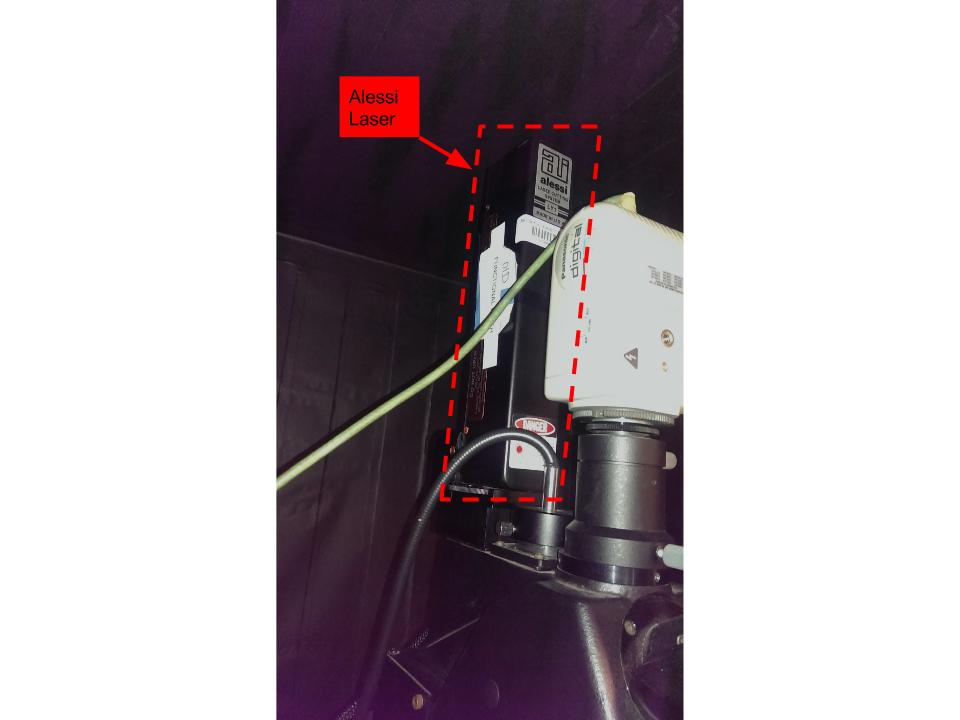
\includegraphics[height=.4\textheight]{laser_02}
                \centering
                \caption{ The Alessi LY1 infared cutting laser housed in the probing station. }
                \label{fig:laser_02}
            \end{figure}

            \begin{figure}[h] 
                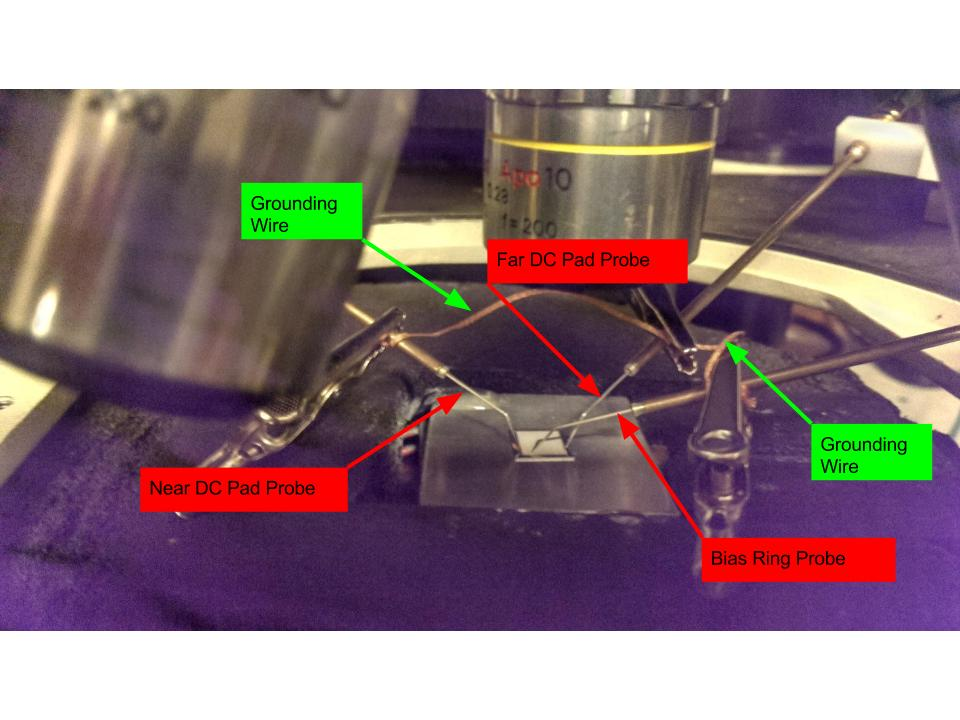
\includegraphics[height=.4\textheight]{probe_tips_00}
                \centering
                \caption{ The standard laser injection setup, with three probes connected by a piece of copper wire. }
                \label{fig:probe_tips_00}
            \end{figure}

            %power supply circuit
            The probe at the front of the platform (the "bias probe", as it will be used to bias the sensor) should have a standard coaxial cable connecting it to the ground terminal of the splitter box. The high voltage ouput of the splitter should be connected to the probe station chuck. And the Triaxial input to the splitter should be attached to a power supply capable of ouputting a kilovolt. 
            
            %copper wire loop
            The probe barrels of all three probes need to be attached to each other with small pieces of copper wire and aligator clips. The reason for this is to ensure that everything is properly grounded. If you fail to do this, data you receive on the oscilloscope will likely be skewed in some fashion. Additionally, you want to make sure that the copper wire loop is as small as possible. The loop acts like an inductor that introduces unwanted noise to the system. Minimizing the size of the loop reduces noise it produces.

            %voltage dividers
            Two of the probes need special voltage dividers attached to them. By my convention, these are always the two probes at the back of the station (in general, they are the probes you intend to touch down on the dc pads). Unscrew the coaxial cables from the probe barrels, and attach the voltage dividers in their place. There are two voltage dividers, labelled "1" and "2". It \textit{does} matter which probe they are plugged into. The voltage divider labelled "1" should be plugged into the "near" dc-pad probe, and "2" should be plugged into the "far" dc-pad probe. "Near" and "far" are terms that will be used many times, and refer to the dc-pad nearest to the sensor's bias resistor, and the dc-pad furthest from the bias resistor. More on this in the next section. By my convention, "1" is always plugged into the left probe, and "2" into the right probe.
            
            \begin{figure}[h] 
                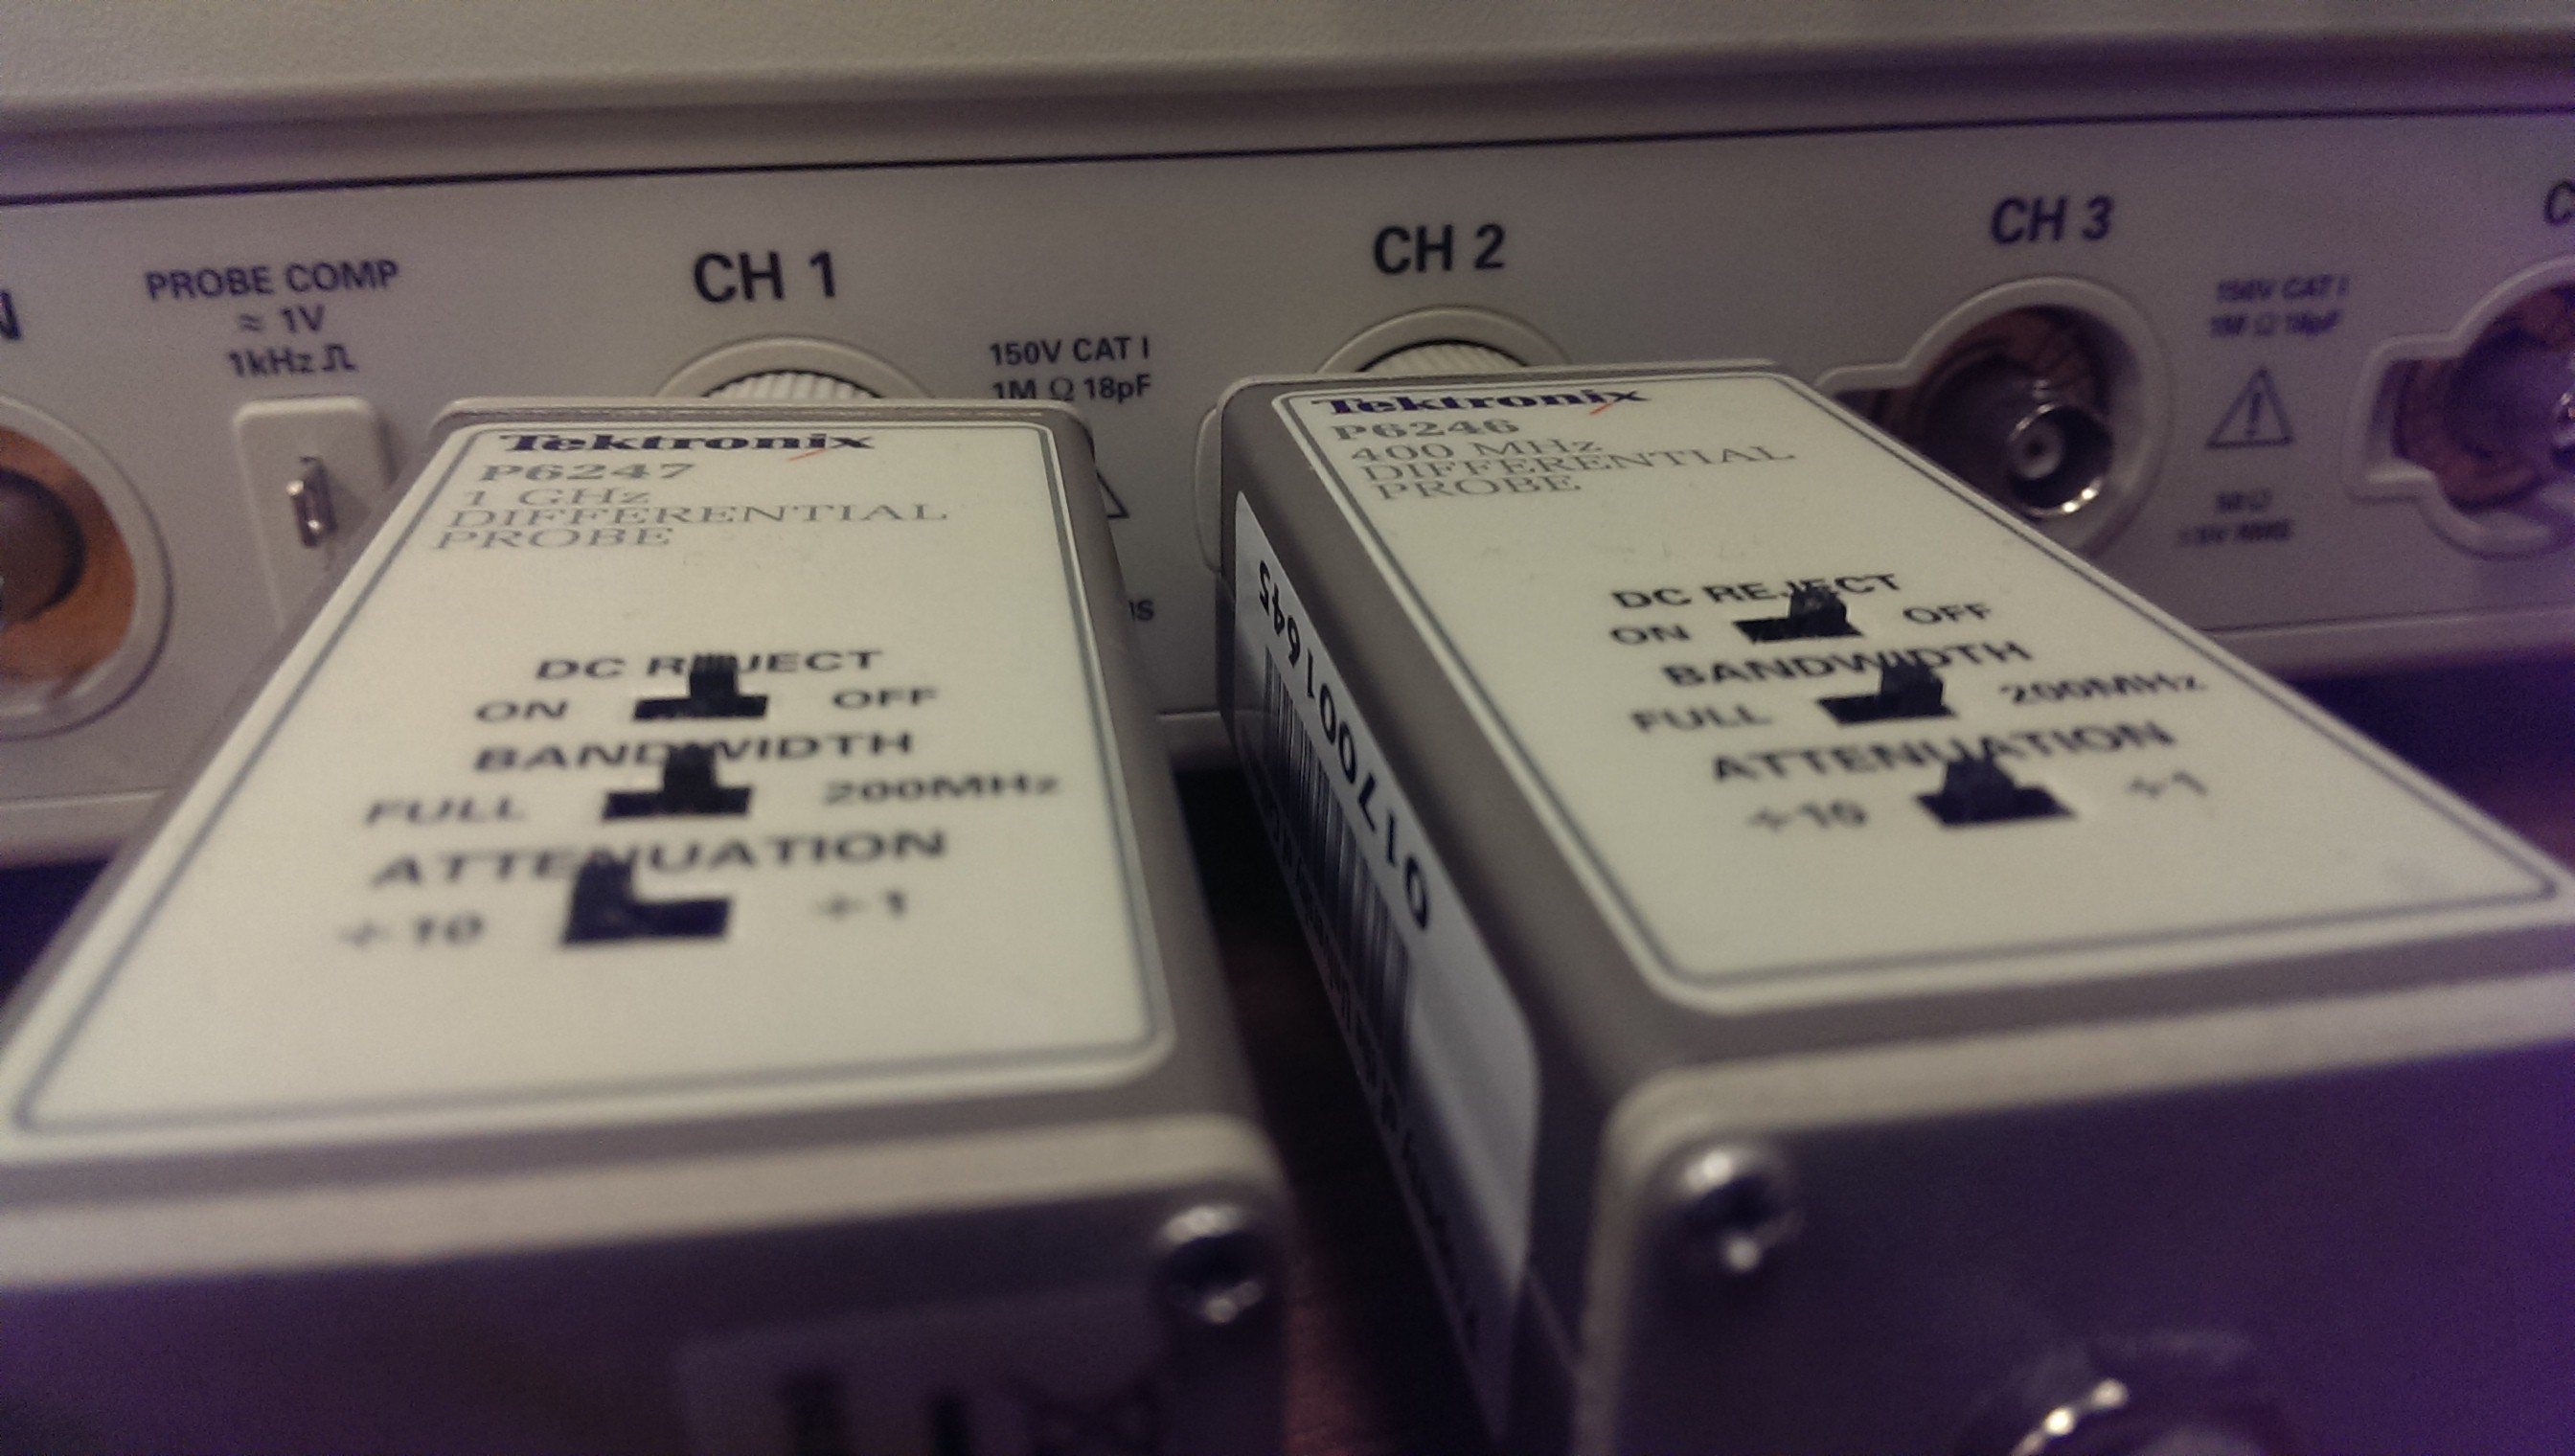
\includegraphics[height=.4\textheight]{diff_probe}
                \centering
                \caption{ A picture of the two differential probes. Note that their settings are the same and are set to, from top to bottom: DC REJECT = OFF; BANDWIDTH = 200MHz; and ATTENUATION = $\div$10. }
                \label{fig:diff_probe}
            \end{figure}

            %differential probes
            The reason for these voltage dividers is to protect the Tektronix differential probes. The differential probes are only rated to 25 volts, while the sensor's dc pads can output several hundred volts. The differential probes need to be plugged into the voltage dividers on one end, and into the Tektronix TDS 5054 Oscilloscope (CH1 and CH2) on the other. The settings for both differential probes should be set as shown in figure \ref{fig:diff_probe}. That is, "DC reject" should be set to off, "bandwidth" should be set to 200 MHz, and "attenuation" should be set to "divide by 10".

            \begin{figure}[h] 
                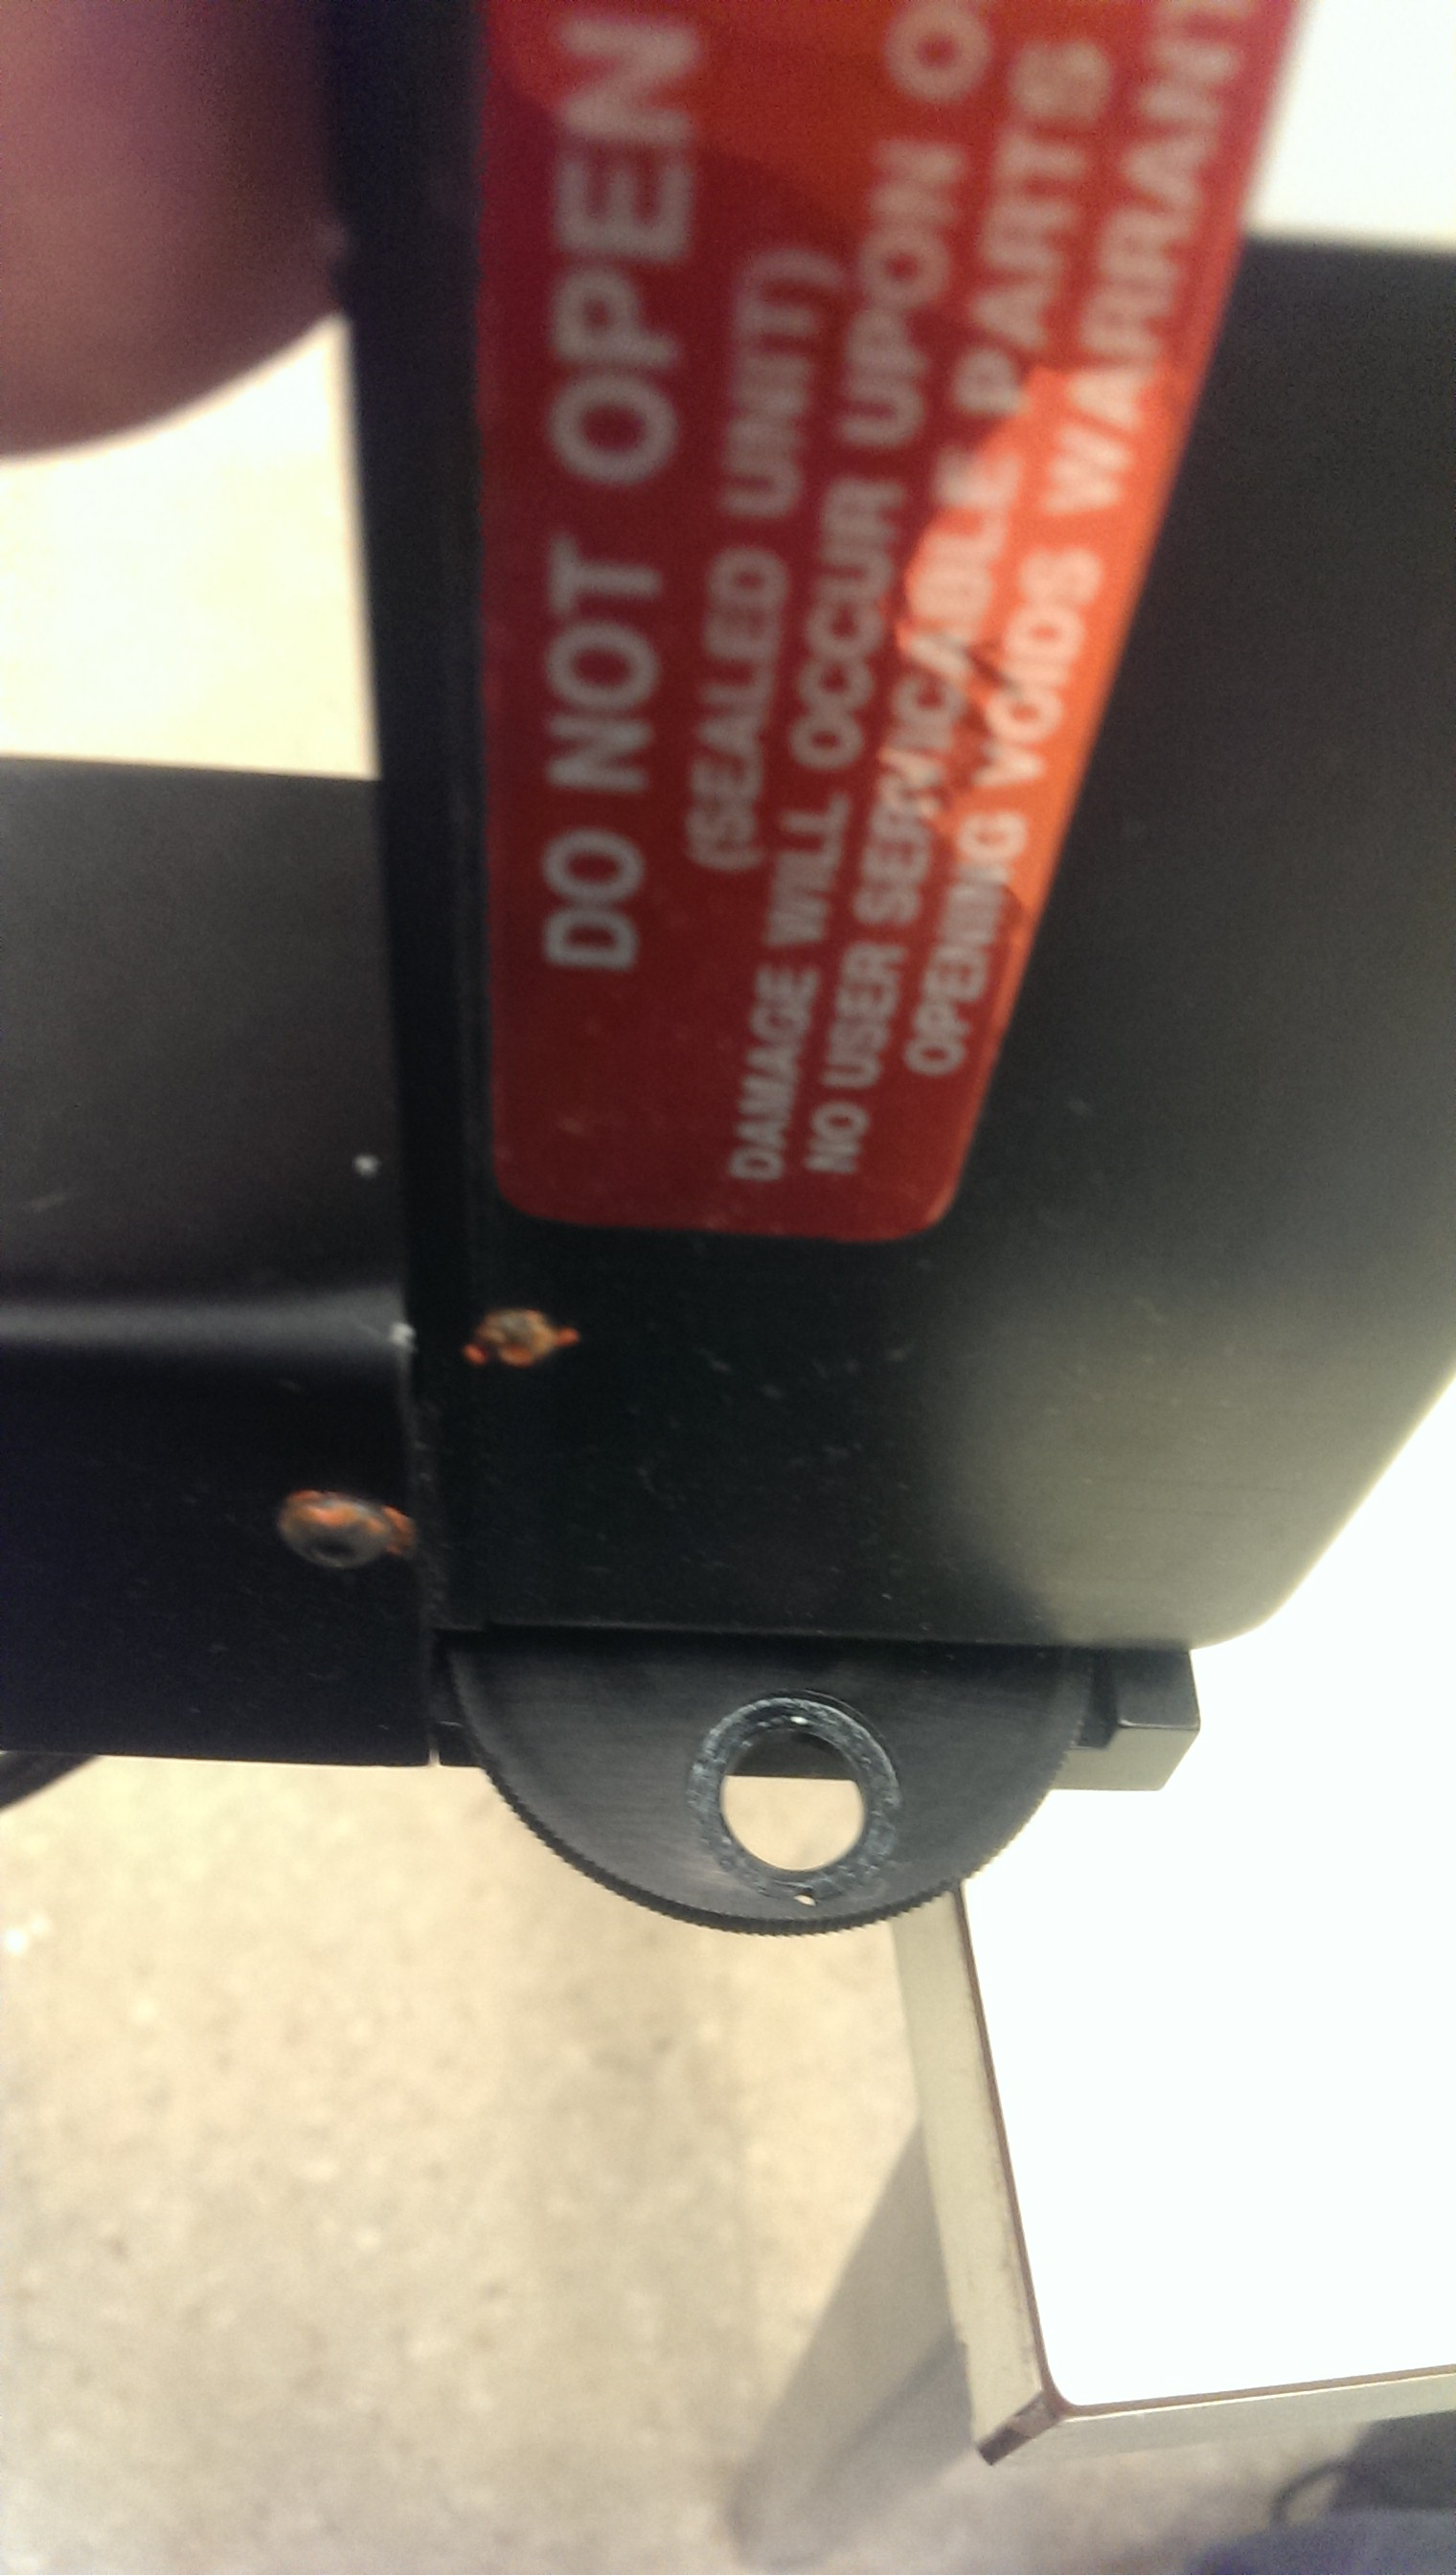
\includegraphics[height=.4\textheight]{laser_00}
                \centering
                \caption{ A view of the oscilloscope filter cylinder from above. }
                \label{fig:laser_00}
            \end{figure}

            %Laser filter
            The last step before getting a sensor is making sure the laser is ready. Find the neutral density filter cylinder (figure \ref{fig:laser_00}) and make sure the filter you intend to use has been placed in the cylinder and rotated into position in front of the laser beam. Be very careful to make sure you are using one of the more powerful filters, as using the weaker filters will result in damage to the sensor. Locate the the laser power box, insert the safety key, and arm the laser. Do not turn the laser on yet. It is now time to get the sensor ready.

            \begin{figure}[h] 
                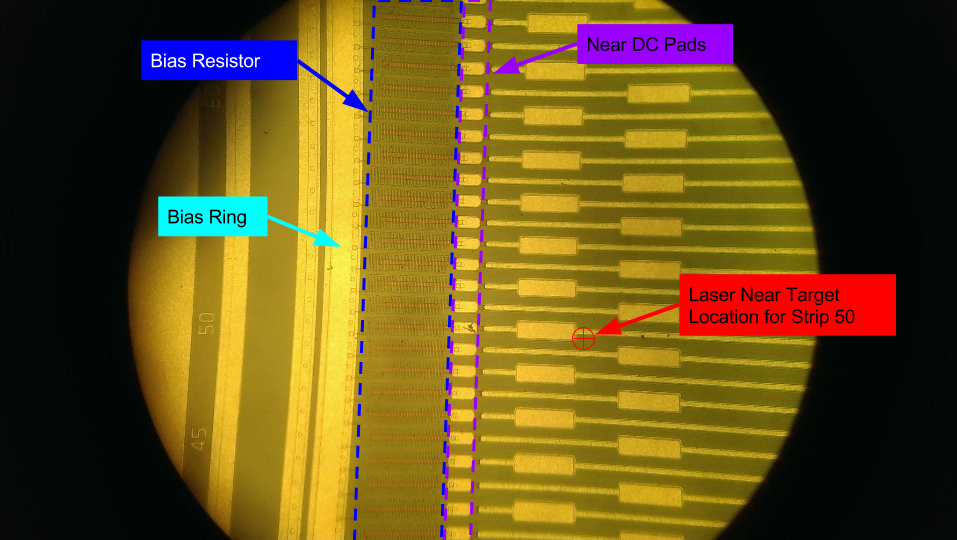
\includegraphics[width=\textwidth]{sensor_near}
                \centering
                \caption{ A view of the near side of an ATLAS07 BZ4A sensor, with key areas for laser injection experiments highlighted. }
                \label{fig:sensor_near}
            \end{figure}

            \begin{figure}[h] 
                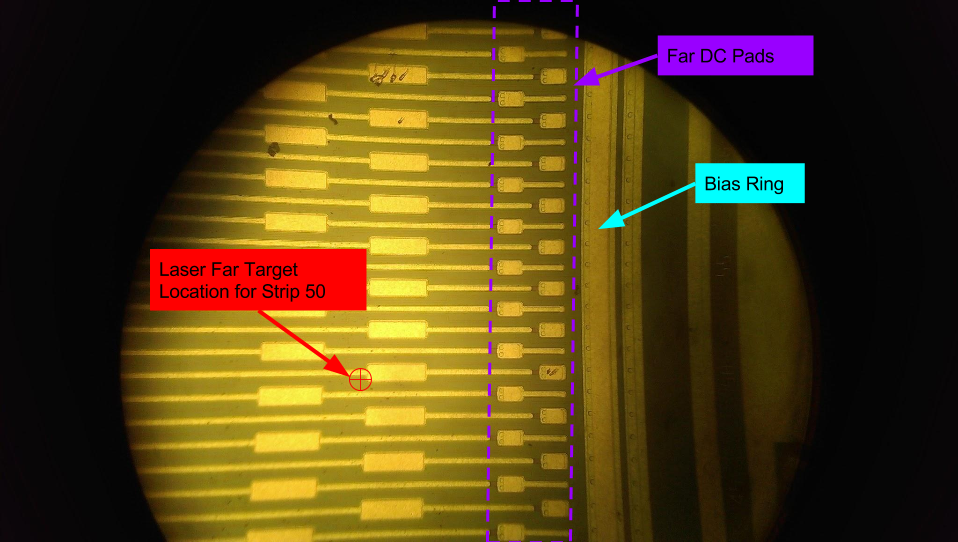
\includegraphics[width=\textwidth]{sensor_far}
                \centering
                \caption{ A view of the far side of an ATLAS07 BZ4A sensor, with key areas for laser injection experiments highlighted. }
                \label{fig:sensor_far}
            \end{figure}

        %touch down on sensor pads, aim laser, turn laser on
        \section{ Readying the Test Sensor }
            %place sensor, touch down
            Place the test sensor onto the chuck. By my convention, I always make sure that the bias resistors, visible in figure \ref{fig:sensor_near}, are on the left. Time to touch down. Pick a strip number. The "near" probe should touch down onto the dc-pad nearest the bias resistor on that strip, and the "far" probe should touch down on the dc-pad furthest from the bias resistor on that strip. The bias probe should of course touch down on the bias ring.

            \begin{figure}[h] 
                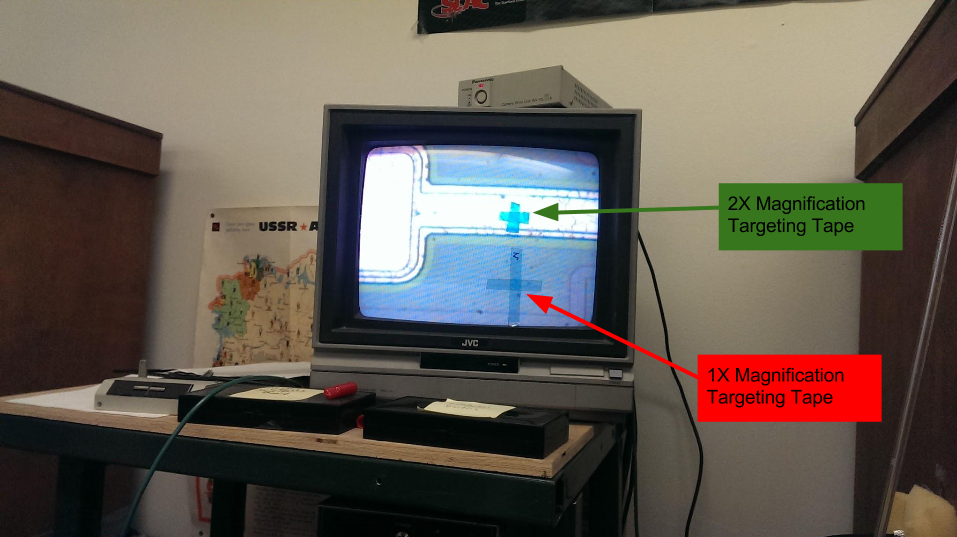
\includegraphics[height=.4\textheight]{monitor}
                \centering
                \caption{ Picture of the viewing screen for the microscope. Two crosshairs are marked on the screen with tape, designating where the laser will fire at a specific magnification level (using the APO SL50 lens). }
                \label{fig:monitor}
            \end{figure}

            %aim ze lazer
            The last step before you can start testing is to aim the laser. This must be done using the high (APO SL50) magnification lens, but \textit{not} using the extra 2X magnification. There are two locations we typically aim the laser at, near the bias resistor and far away from the bias resistor. Figures \ref{fig:sensor_near}, \ref{fig:sensor_far}, and \ref{fig:monitor} show exactly where I usually aim the laser. Precise aiming of the laser is accomplished using the CRT microscope viewing monitor. There are two pairs of tape on the screen, which act as crosshairs. One pair is for when the microscope is at 1X magnification, the second pair for 2X magnification (only used when you intend to actually cut things). With the laser aimed, turn off the viewing light and close up the probe station (the light will break the sensor when biased, and the laser will not operate with the station open).

        %FIRE ZEE LAZER!!! (every 3 s. max...). Filter out double peaks. Watch for damage
        \section{ FIRE ZE LAZER!!! (carefully): \\ Laser and Oscilloscope Operation }
            %warning
            Before we go any further, I should make something clear: You are testing a very fragile and sensitive piece of electronic equipement that can be damaged with a misdirected flashlight. You are about to shoot directly at it with a laser \textit{that can make craters in metal}. In my time doing these tests I have amassed an entire graveyard of sensors which were damaged or destroyed because of this laser. I cannot stress enough how important it is to be careful and patient with this part of the experiment. Negligence \textit{will} result in your sensor being rendered untestable at best, and outright destroyed via laser ablation at worst (figure \ref{fig:crater}).

            \begin{figure}[h] 
                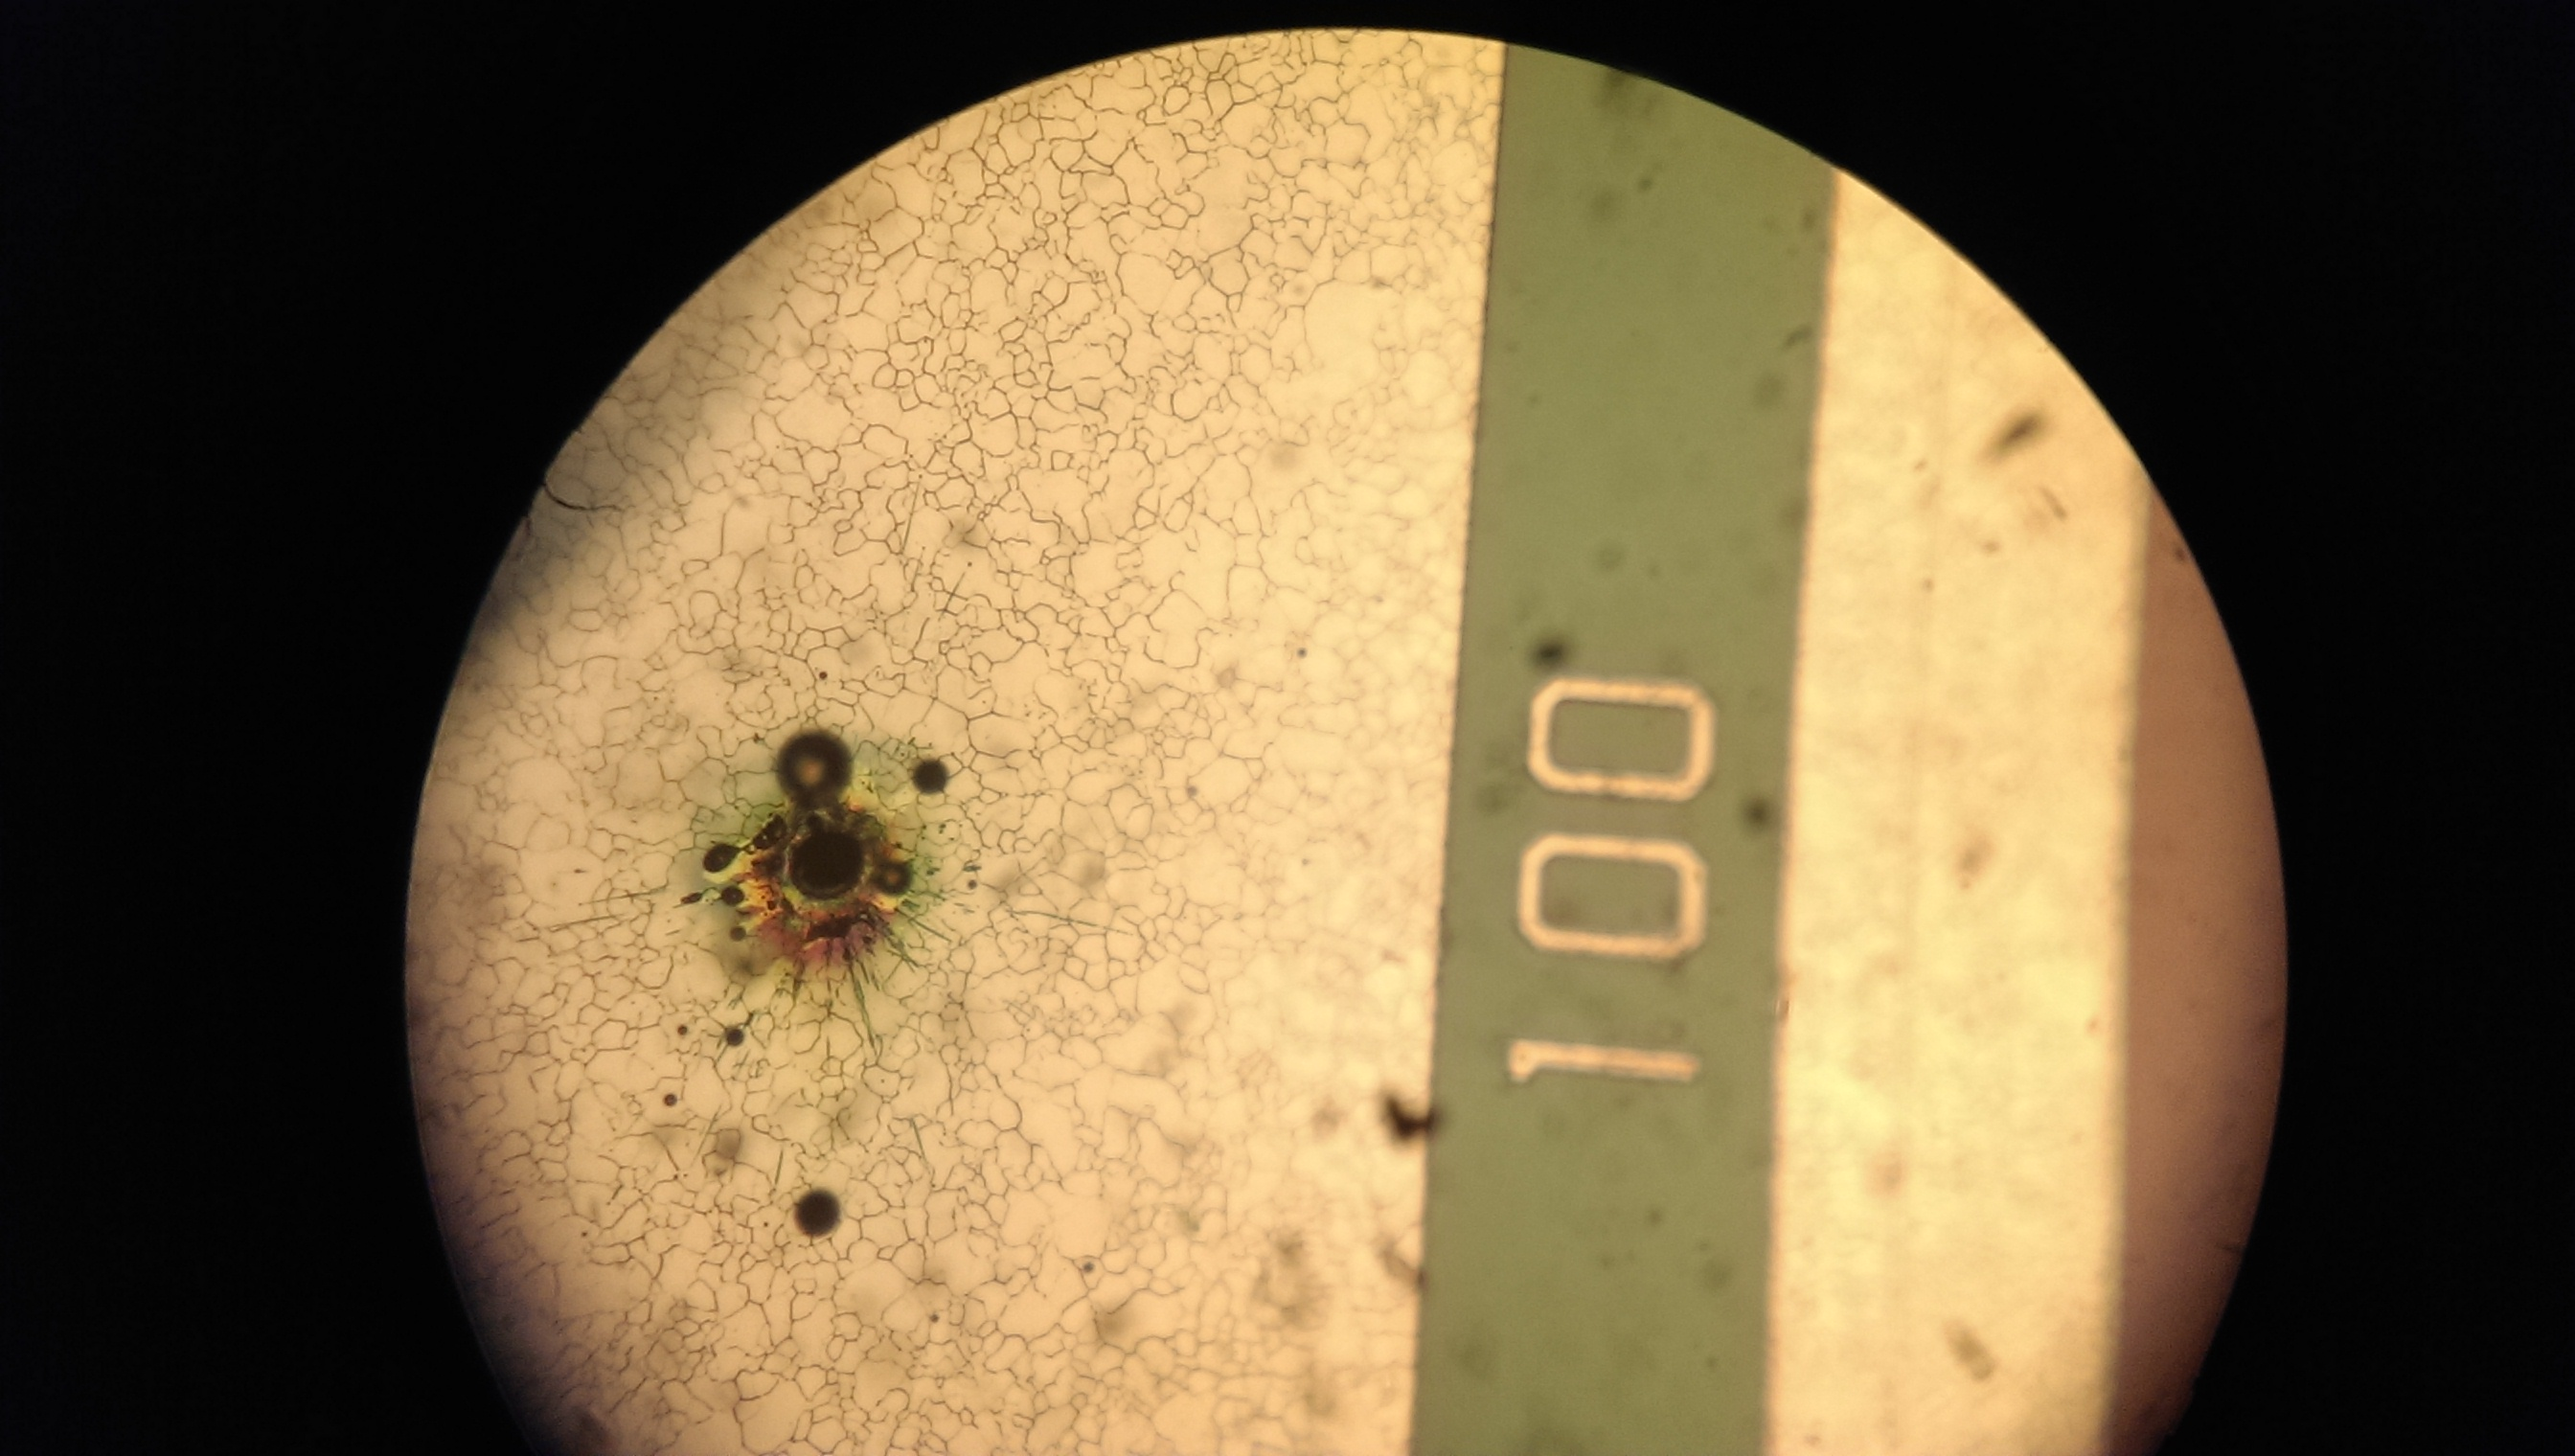
\includegraphics[height=.4\textheight]{crater}
                \centering
                \caption{ This is an ablation crater from a single shot of the laser at full power and no filter. Please do not do this to a working sensor. }
                \label{fig:crater}
            \end{figure}

            %turning on the laser
            With that out of the way, the first thing to do is to turn on the sensor power supply. Assuming you wired everything up correctly, you want to bias the sensor with negative voltage. I've found that the best place to start is by biasing to -50 volts, as the laser is less likely to damage the sensor at this voltage. Once you've assured yourself that you have a solid bias connection, it is time to turn on the Alessi Power Supply. As of writing this thesis, you will want to set the laser power to 511. As mentioned in section \ref{sect:mystery}, the laser power that we can operate at does not seem to be consistent, and you may need to use a different value. The important thing is to not go too high. Using too large a value here is guaranteed to break the sensor.

            \begin{figure}[h] 
                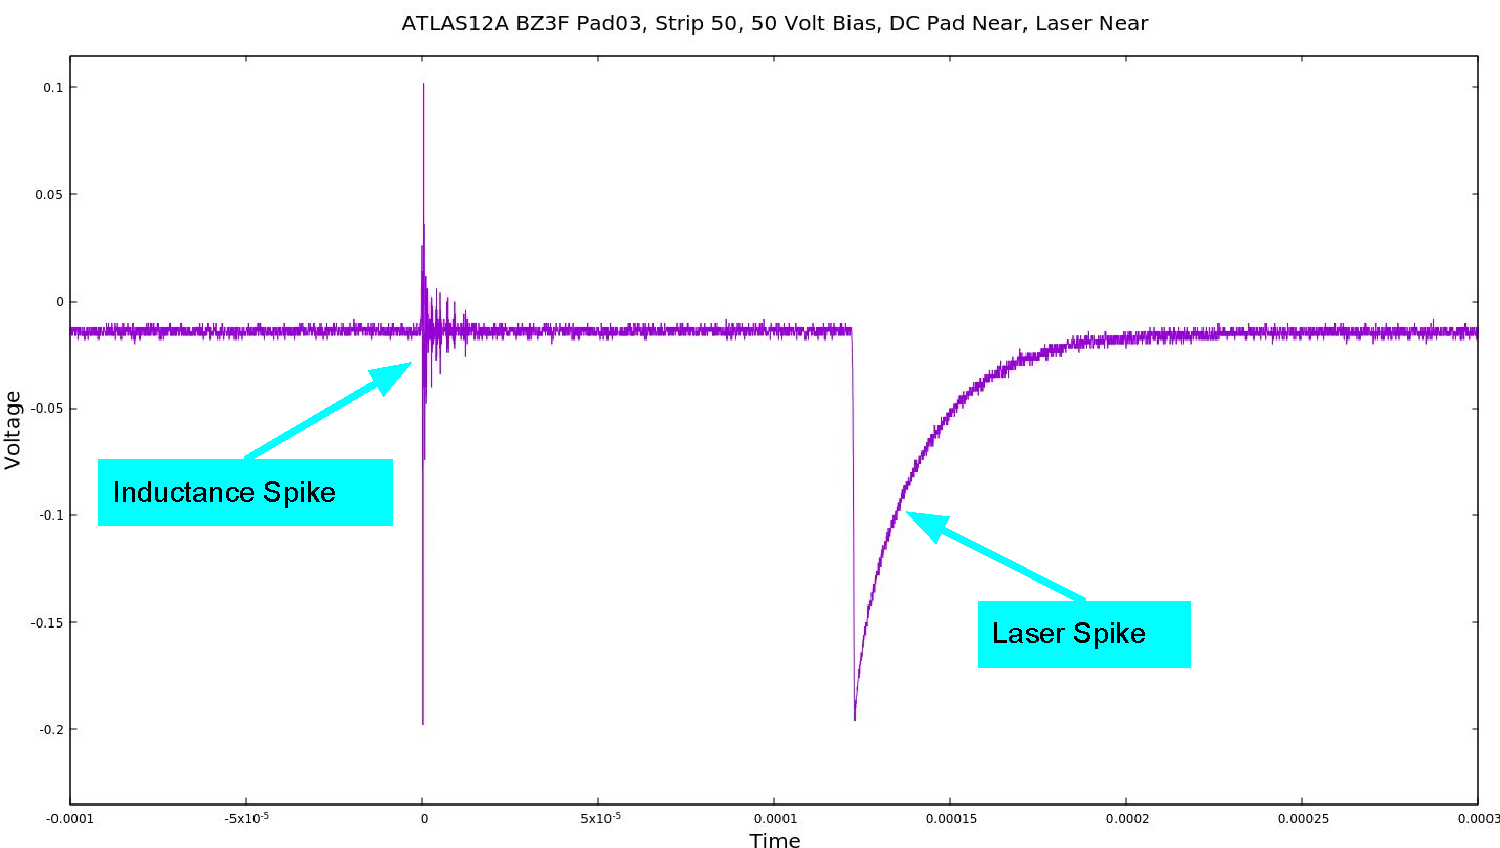
\includegraphics[height=.4\textheight]{50V_spike}
                \centering
                \caption{ A typical example of the raw output of a laser induced voltage spike, using a 50 volt bias. }
                \label{fig:50V_spike}
            \end{figure}

            %initial test fire
            With the laser power set, you can now finally fire the laser... every 3-5 seconds. For the safety of both the laser and the sensor, you are prohibited from firing the laser any more than once every three seconds. Because I like to be especially cautious, I always prefer to fire only every five seconds. The laser can be triggered with the trigger switch on the laser power supply or, more conveniently, with the attached foot peddle. Fire the laser and watch the oscilloscope. If you are lucky, you should see a sudden spike (or pair of spikes) like in figure \ref{fig:50V_spike}. However, the Alessi laser is nothing if not inconsistent, which mean you may have to fire the laser several times (once every 3-5 seconds...) before you see such a spike. It is not unusual to have to wait up to 20 shots before seeing a spike. If you do not see a spike after that many laser triggerings though, you should check your probes' connections to the dc pads.

            \begin{figure}[h] 
                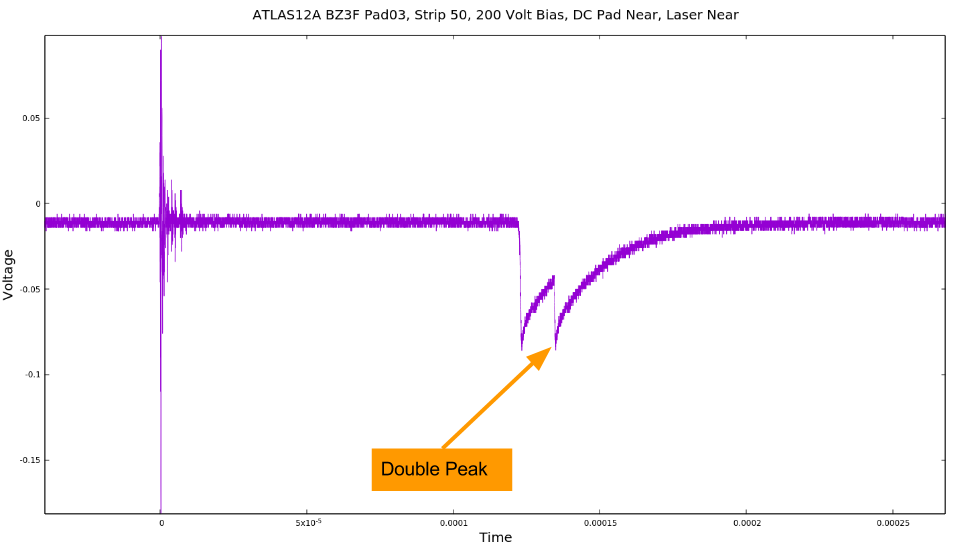
\includegraphics[height=.4\textheight]{double_peak}
                \centering
                \caption{ A typical double spike, resulting from the laser firing two pulses in short succession. They are not harmful to the sensor, but you cannot use the data from them. }
                \label{fig:double_peak}
            \end{figure}

            %what to watch for
            Upon seeing a pulse and confirming that your oscilloscope probes are properly touched down, you can begin recording data. Fire the laser as many times as you need, at whatever bias voltages you need. While doing so however, pay very close to attention to both the shape of the spikes you see, and the leakage current running through the sensor (visible on the power supply). There are two things that can go wrong with the spike shape. The first is that you can get a "double peak", as visible in figure \ref{fig:double_peak}. A double peak (and at high enough laser powers a triple peak) like this indicates that the laser fired twice in a very short period of time. As our experiments are always concerned with only single pulse spikes, you need to throw away these double peak pulses. 

            \begin{figure}[h] 
                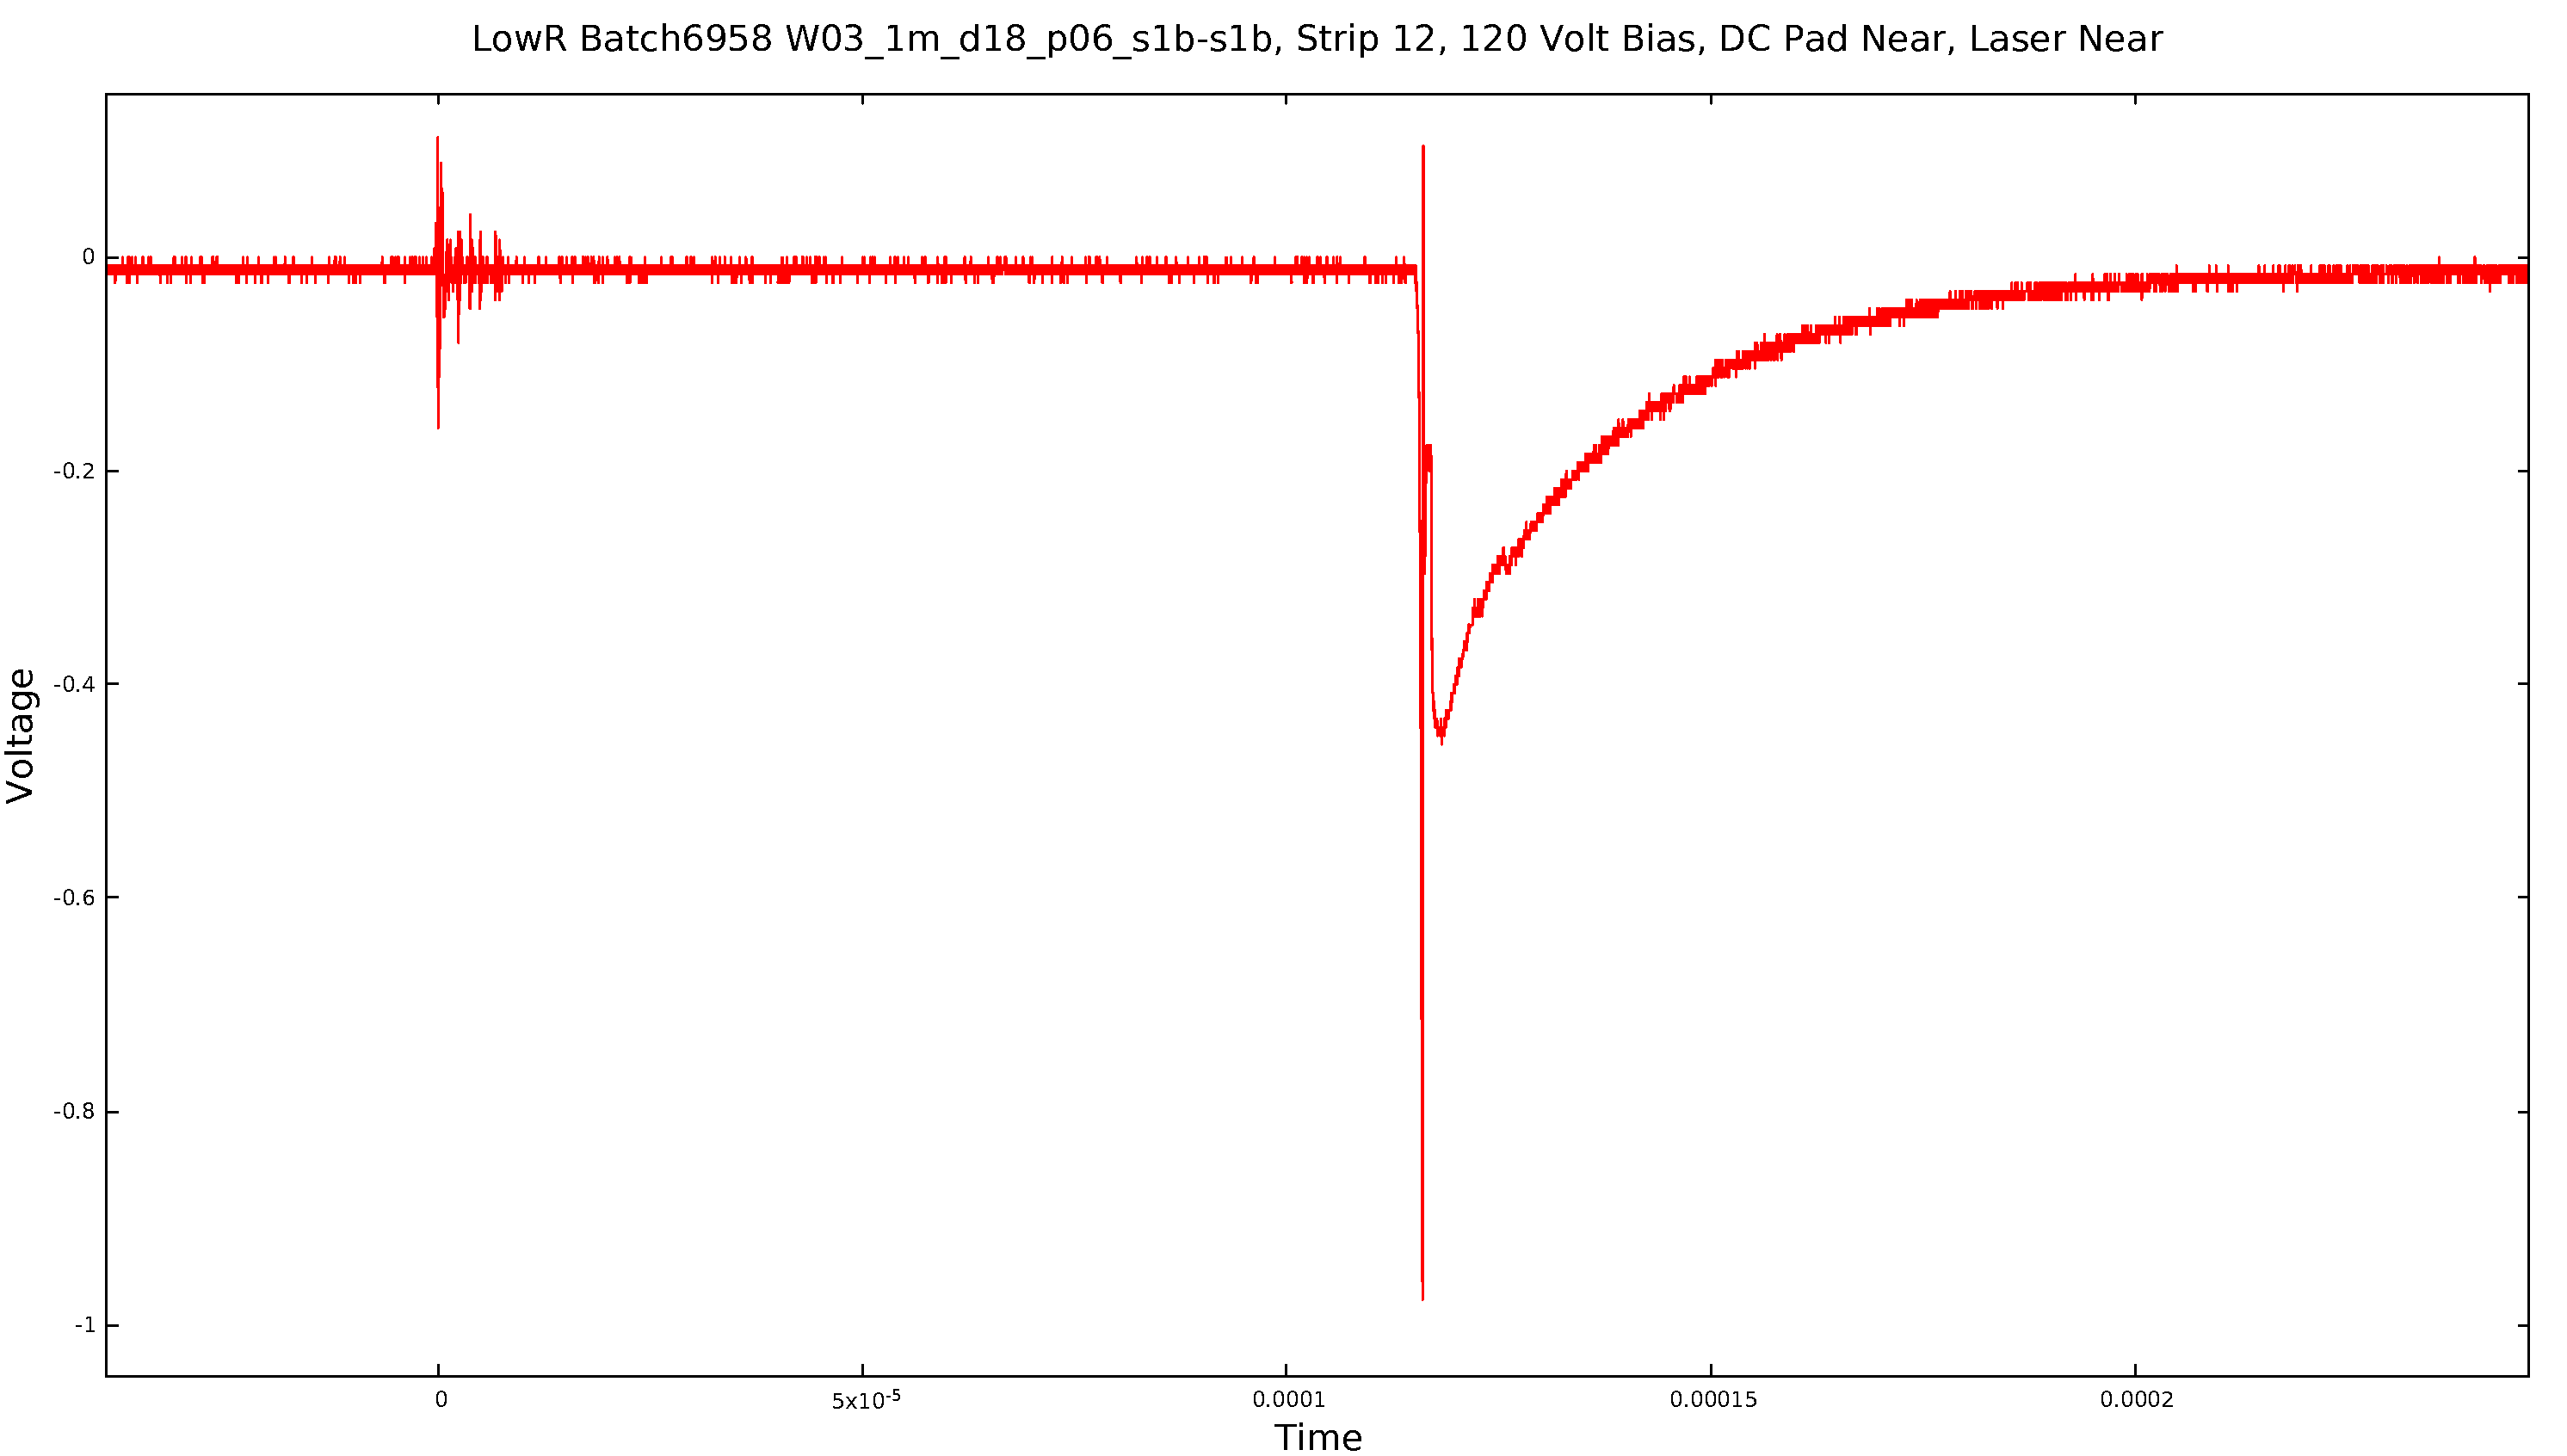
\includegraphics[height=.4\textheight]{damage_spike}
                \centering
                \caption{ A typical damage spike. Note the distinctive vertical line immediately preceding the more normal looking voltage spike. }
                \label{fig:damage_spike}
            \end{figure}

            \begin{figure}[h] 
                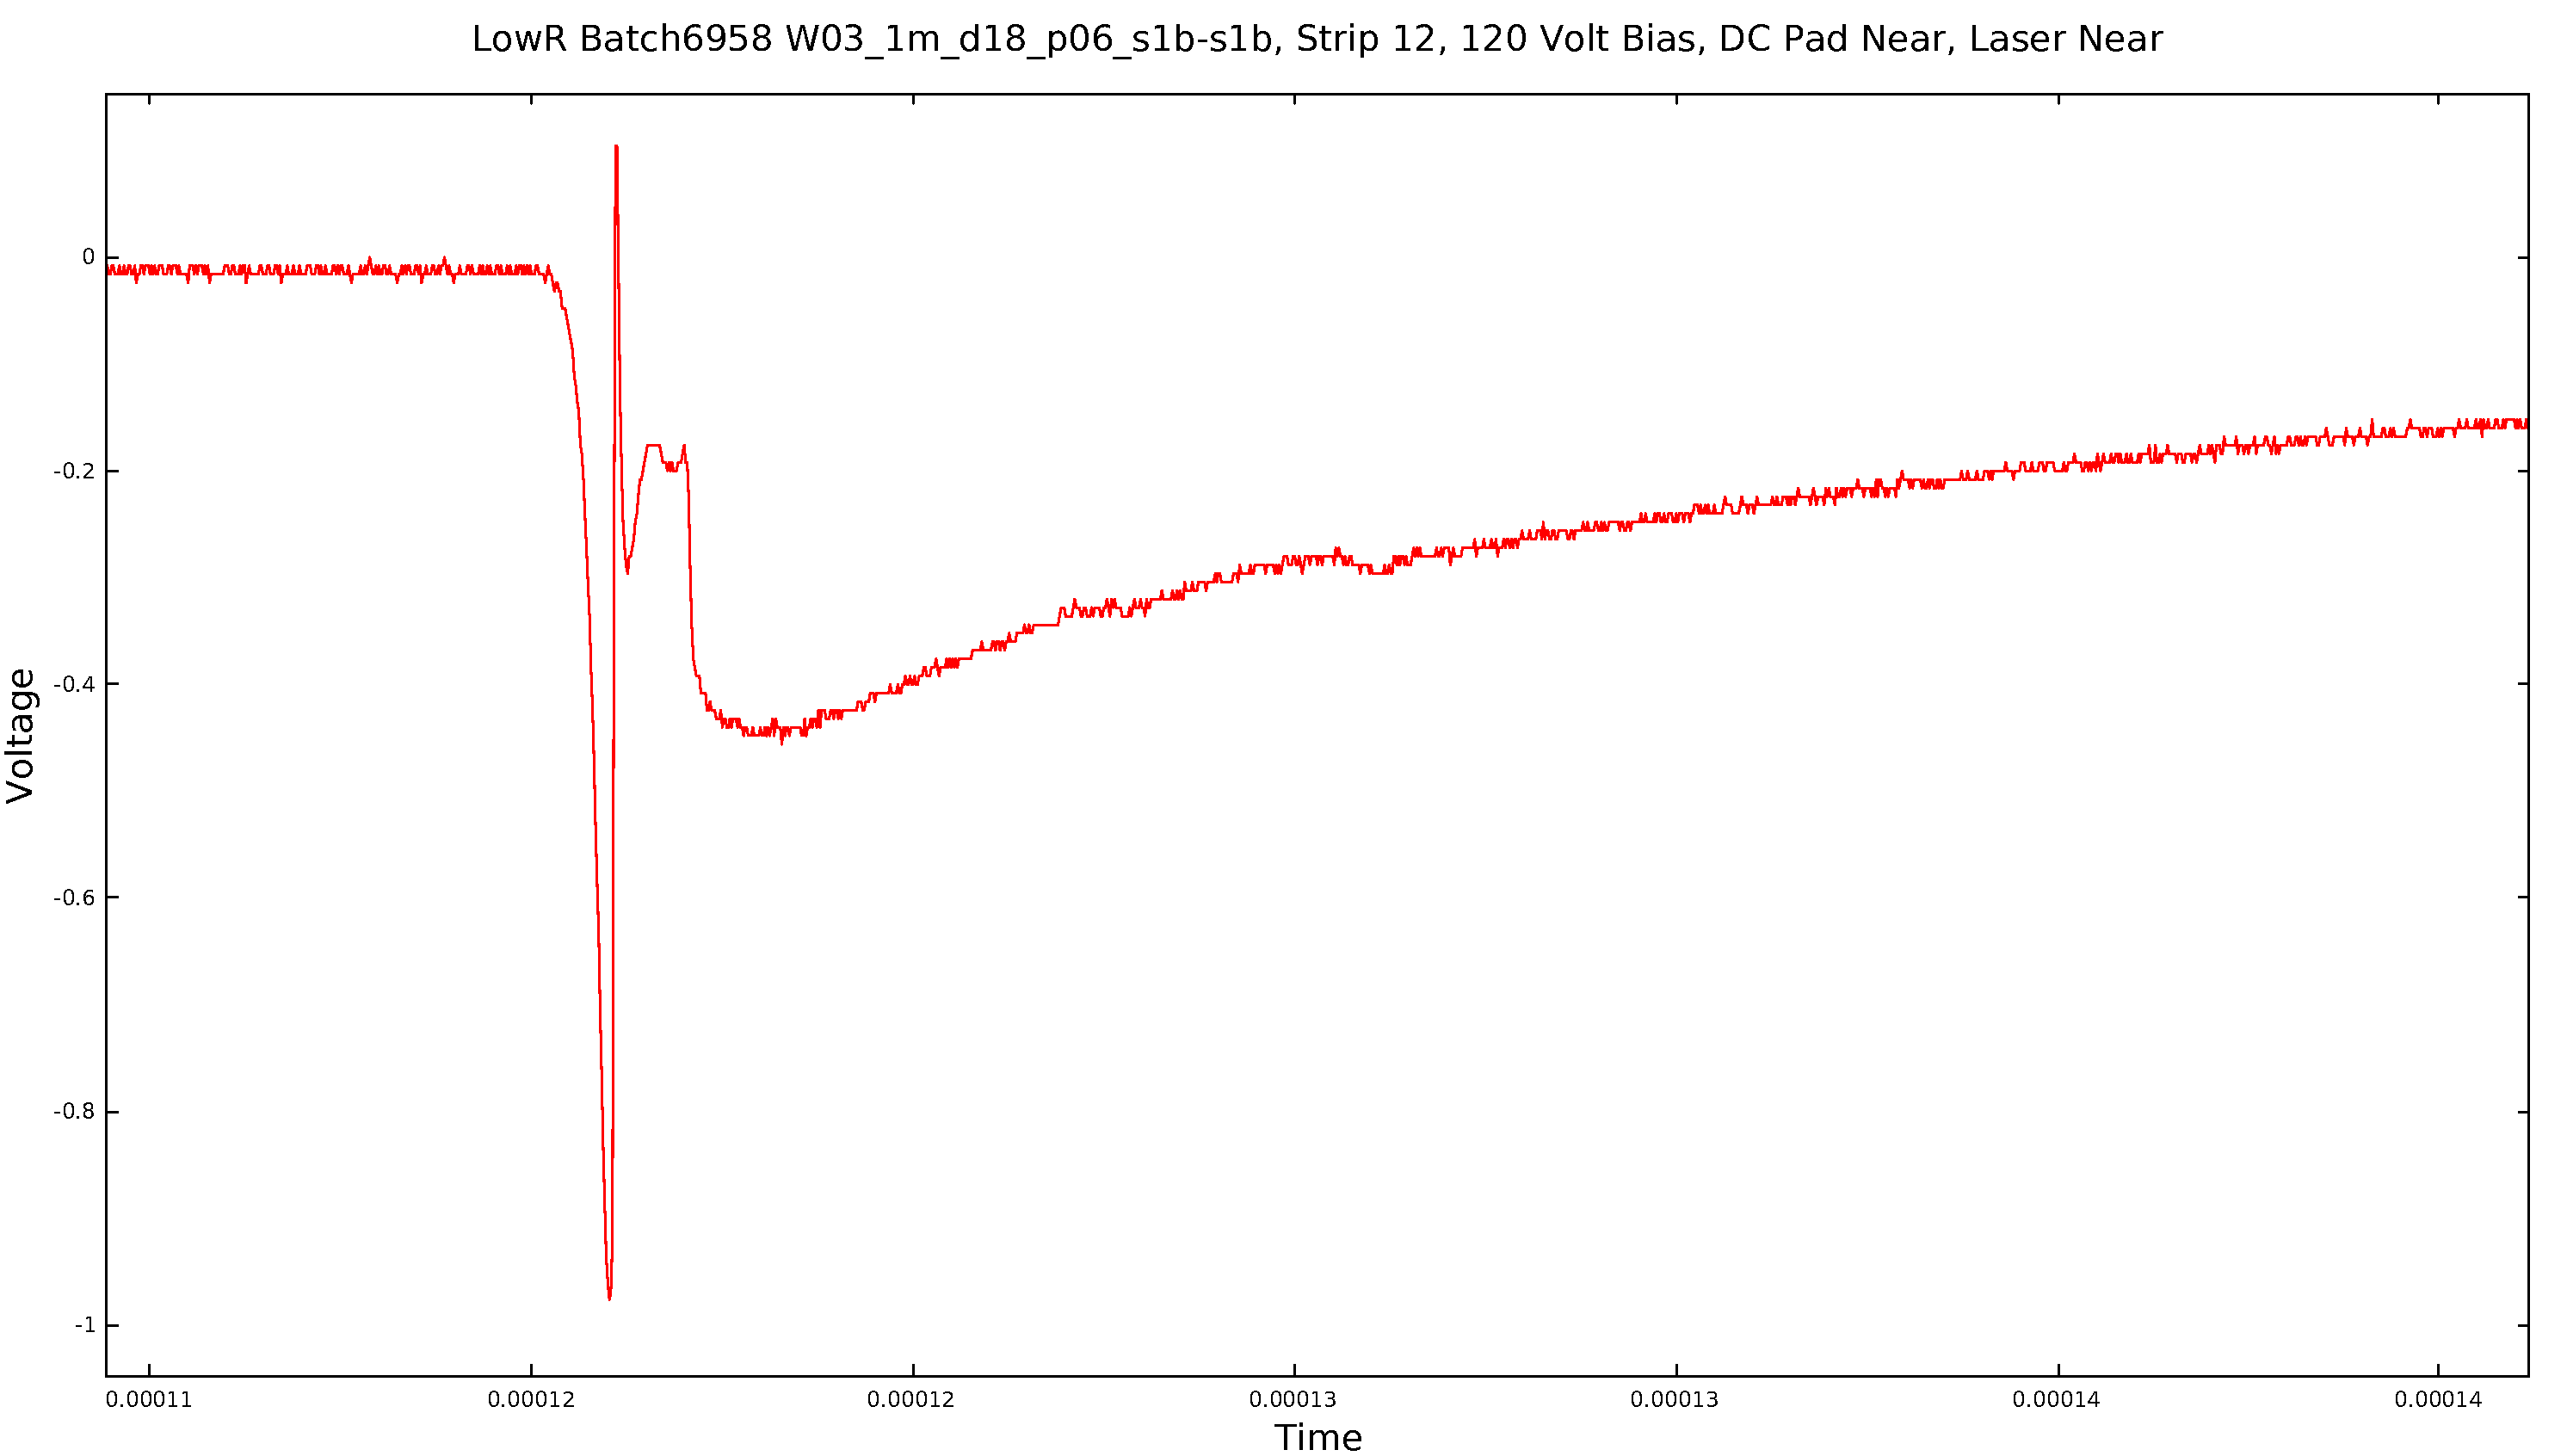
\includegraphics[height=.4\textheight]{damage_spike_zoom}
                \centering
                \caption{ A typical damage spike, a bit zoomed. At this scale, the telltale vertical line resolves into a very sharp negative peak, before rising into a positive peak, and then regularizing to a more normal voltage spike. The positive aspect of the spike is the most noteable, as a negative reverse biased sensor should never output positive votage. }
                \label{fig:damage_spike_zoom}
            \end{figure}
            
            %marks of death
            The second pulse shape to watch for, which I refer to as a damage spike (figures \ref{fig:damage_spike} and \ref{fig:damage_spike_zoom}, is much more concerning. An occurance of one of these indicates that you are beginning to damage the strip you are shooting at. Note, that this damage is permanent, but is limited to that strip and its neighbor strips (see appendix \ref{sect:ptp_study} for more detail). If you see a damage spike, STOP. You are officially playing russian roulette with the sensor, and any laser shot from this point on risks globally damaging the sensor. With that said, the issue of global sensor damage leads us to the second aspect you need to pay attention to while testing sensors: the leakage current.

            %leakage current
            After every pulse of the laser, take a glance at the leakage current through the sensor. If, upon triggering the laser, the leakage current suddenly jumps up several orders of magnitude, STOP. The sensor has been globally damaged. Technically the sensor is still usable, but I would strongly recommend that you no longer use it for laser injection testing. Firing the laser at such a sensor will only cause the leakage current to rise higher, eventually maxing out the power supply's maximum compliance rating and rendering the sensor completely unusable. Assuming that you manage to skirt disaster though, and are able to export your data, we need to look at some post-processing.

        %python!!!
        \section{ Post-Experiment Analysis }
            %initial sweep: smooth data, remove offset
            The post-processing of the data for this experiment is fairly starghtfoward, and ultimately amounts to plotting the peak voltages of the various measurements against the bias voltage those measurements were taken at. There are a couple of caveats to obtaining this value however. The first step in this process is to smooth out the data and set a proper baseline. Smoothing the data out is a straightforward process that simply uses a running mean to make the data less erratic. As for the baseline, the voltage going through the probes/differential probes/oscilloscope tends to be very slightly offset from zero. As such we need to shift all the data points slightly to get the proper relative values. This is done by \textbf{assuming} that the first several data points (my algorithm uses the first 5\%) are flat, with no pulse data. When configuring the oscilloscope, you should ensure that the trigger point is not too far to the left, so that this assumption remains true.

            \begin{figure}[h] 
                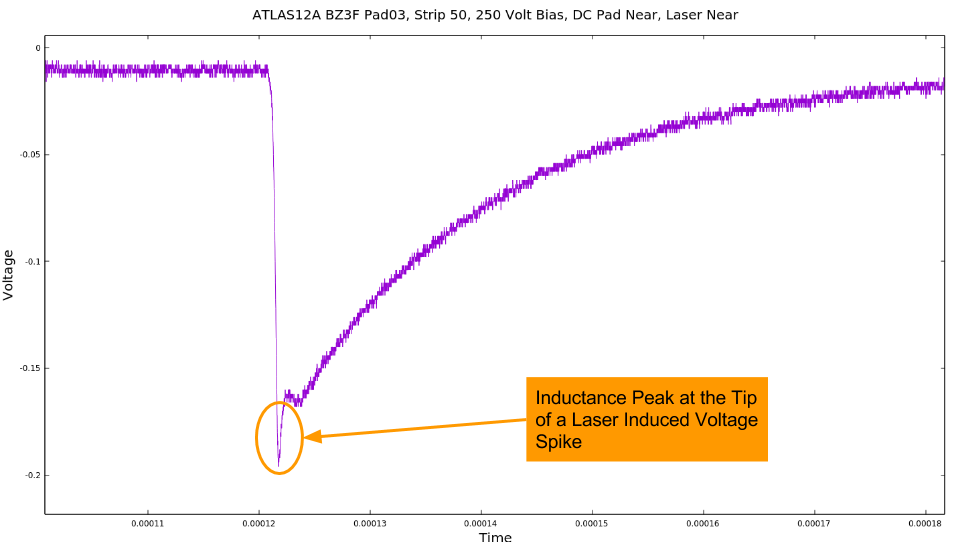
\includegraphics[height=.4\textheight]{inductance_peak}
                \centering
                \caption{ A small inductance spike at the tip of a standard voltage spike. These are unavoidable with the current setup, and so must be removed while processing the data. }
                \label{fig:inductance_peak}
            \end{figure}

            %remove inductance spike, find laser pulse
            Once the data is smoothed out and corrected for the dc offset, the next step is to sort through the measurement data from a pulse and locate the actual spike. Due to the way the experiment is setup, firing the laser causes inductance in the oscilloscope probes, leading to a small but sharp spike being captured by the oscilloscope seen in figure \ref{fig:inductance_peak}. In fact, in the majority of cases, this inductance spike is what the oscilloscope triggers off of. In order to avoid confusing the analysis, this inductance spike is removed. Fortunately, this is a simple matter, because while the pulse caused by the laser is purely negative, the inductance spike is both negative and positive. With the data now appropriately cleaned up, the laser pulse can be easily identified by simply being the most negative voltage of the data.

            %laser peak clipping
            Finding the laser peak is not quite the end though. Due to another quirk of the setup (again, possibly because of inductance...), the peak that appears on the oscilloscope is higher than the actual maximum voltage going through the strip of the sensor. It was found in previous studies that this additional perceived voltage is related to the rise time of the laser pulse; the shorter the rise time, the higher the pulse. Calibrations were performed to accurately measure this dependence. We use the data from those calibrations in combination with the rise time of the laser pulse in order to determine how distorted the laser pulse tip is. Finally, the laser pulse is then trimmed down by an appropriate amount, and the finished peak data can be used for further study.

            



    \chapter{ What I Have Previously (Unsucessfully) Tried\\ AKA: What Not To Do }
        \section{Initial Non-PTP Tests}
            The very first laser injection tests I performed were on ATLAS07 BZ6 sensors. These initial tests were actually a mistake, as the BZ6 model does not posses a notable PTP structure. As will be seen in the following section though, PTP equipped sensors are very problematic, especially when compared to sensors which do not have a PTP structure. As such, this first set of tests provides a useful comparison.

            The first set of tests were performed using the NENIR510B neutral density filter, with the laser power set to 509. They were performed on ATLAS07 BZ6, wafers 50 and 51 using the setup described in section \ref{sect:methods}. All tests were performed up to a bias voltage of -200 volts, and all tests completed without any issue. No damage spikes were ever seen, and the leakage currents through the sensors were the same as before the tests were started. The peak voltage versus bias voltage plots for the sensors are shown in figures [TODO: get plots from:
            %150805_atlas07_w50_BZ6-P12 and 150806_atlas07_w51_BZ6-P12
            ]. What should be noted in these plots is that the voltage curve never flattens out. The peak voltage continues increasing almost linearly with the bias voltage across the entire voltage range. This unborken linear dependence is completely expected in the BZ6 model sensors, as they lack any significany PTP structure.

        \section{Standard Laser Injection Testing} \label{sect:std_tests}
            The next round of tests used sensors equipped with a strong PTP structure. Specifically, the ATLAS07 BZ4A model sensor, the ATLAS12A BZ3C model sensor, and, very briefly, a LowR sensor. I should note that, at some point during these tests \footnote{Specifically, the switch may have been done at any point between the first ATLAS07 BZ6 test from earlier, up to the ATLAS12A BZ3C W757 Halfmoon: Left P14 tests.} I switched the neutral density filter from the NENIR510B model, to the weaker NENIR504B model. The reason is that the 510 did not actually fit the laser, and scraped against the holder everytime it was rotated. I'm kicking myself for not writing down when I swapped out the filters, but future studies (specifically, those in section \ref{sect:new_filters}) suggest that it probably did not matter either way, as even the NENIR513B filter was unable to protect the sensors. In any case, these PTP equipped sensors are where we began to see serious problems.
            
            The first sensor to be tested was the ATLAS07 BZ4A W103-P4 sensor. The incomplete results of this sensor are shown in figure [TODO: get plots from:
            %150901_atlas07_w103_bz4a-p4. Or just use the plots in the "useful" directory
            ]. The measurements taken from the near dc pads shows the curve fall-off indicative of the PTP structure activating. Unfortunately, in a pattern that will become depressingly consistent throughout the remainder of the results, we have no data beyond this point, which severely limits the observations we can make about the PTP structure in action. The reason we have no more data is that, while shooting the laser near the near dc pad on strip 75 with a bias voltage of -110 volts, I encountered my first damage peak, visible in figure [TODO: use plots from
            %archive/exluded
            ]. To avoid damaging the sensor I abandoned strip 75 and moved to strip 60, only to encounter another damage peak at -170 volts with the laser shooting by the far dc pad. The exact same thing happened when I moved to strip 20. In hopes that the issue was with this sensor alone, I moved to another BZ4A type sensor. Specifically, to ATLAS07 BZ4A W142-P4. I attempted to push this sensor further than the last, and ignored the damage peaks. Figures [TODO: plots
            %150901_atlas07_w103_bz4a-p4
            ] shows the rather limited results I obtained for my efforts. As I continued firing the laser at the sensor, the damage spikes appeared more and more frequently on the oscilloscope. Beyond this however, there was nothing to suggest the sensor was being damaged \footnote{There actually was damage being done, though special testing is necessary to detect it. See section \ref{sect:ptp_study} for more details.}. That is of course, until I fired the laser one too many times and the leakage current through the sensor instantly jumped from 90 nA all the way to the power supply's compliance setting of 1 $\mu$A. At this point I was forced to cease testing on the sensor.

            With the failure of the ATLAS07 laser injection testing, I attempted to instead do testing on the ATLAS12A sensors. I started with the sensor ATLAS12A BZ3C W757 Halfmoon: Left P14. I followed the same procedure as before, with the results visible in figure [TODO: plots
            %150902_atlas12a_w757_bz3c 
            ]. Despite ATLAS12A BZ3C sensors possessing a PTP structure, the PTP structure's effects are not visible. The reason for this is that the ATLAS12A BZ3C PTP structure activates at roughly 300 volts. As with the previous sensor, I pushed this one too far, and the leakage current jumped to compliance (1 j$\mu$A) at a bias voltage of -200 V.

            Another test on an ATLAS12A BZ3C was attempted, using the ATLAS12A BZ3C W757 Halfmoon: Left P15 sensor. Two changes were made to the setup here. First, I switched out the neutral density filter, swapping the NENIR504B filter for an unmarked black filter\footnote{I performed tests in which I shot the laser at full power through various filters at a dummy sensor, comparing the sizes of the craters made with each filter.. I found that this particular black filter left the second smallest crater of all the filters we had at the time, with only the NENIR510B outperforming it.}(see figure [TODO: pic of black filter]). Second, I upped the laser power from 509 to 511; section [TODO: discuss laser power in introduction] explains why this increase is safe. With that said, the results of this tests are presented in figure [TODO: plots
            %150908_atlas12a_757_bz3c-p15
            ]. The telltale platueing of the peak voltages is just barely becoming visible at the edge of the tested bias voltages, but, just as with the ATLAS07 sensors, I was unable to continue further. At a bias voltage of -200 V and the laser firing by the near DC pad, I began to see damge spikes and decided to cease testing of the sensor. At this point it was apparent that something different had to be done.
            

        \section{Tissue Paper}
            Colin Parker wrote a thesis on these laser injection studies, and in it he discusses the usefulness of the neutral density filters. He concludes that the neutral density filters have no significant effect on the laser \footnote{I should note that this conclusion is misleading. A more accurate conclusion is that the \textit{extremely weak} NENIR501B and NENIR502B neutral density filters he uses have no effect on the laser. The more powerful filters (NENIR 504B, 510B, 513B, 520B, and 530B) most certainly \textbf{do} have an effect.}. He then proceeds to develop a method of testing which uses a variable number of pieces of tissue paper placed directly in front of the microscope lens in order to attenuate the laser. A piece of black paper with a small hole cut into it is then placed between the microscope and sensor, in order to shield the rest of the sensor from the attenuated laser light. A picture of my version of this setup can be seen in figure [TODO: tissue paper setup pic]. I used two pieces of tissue paper, a laser power of 513, and \textit{no} neutral density filter to perform these tests.

            Two sensors were tested using a two tissue setup: ATLAS12A BZ3F W[FIXME]-P2 and ATLAS12A BZ3F W[FIXME]-P3. The data for P3 is shown in figure [TODO: plots
            %150914_atlas12a_bz3f-p03 ; check the ignore folder for pics TODO: also check the strip 25 test to see what happened.
            ]. While the sensor was able to tolerate testing up to -400 volt bias, the results are completely useless. The test on the P2 sensor was not recorded, but merely used to confirm that the behaviour seen in the P3 sensor was not because of a defect in the sensor. The P2 sensor was capable of tolerating laser shots up to -700 volts, but peak voltages stopped increasing beyond a bias voltage of only -5 V, whereupon it displayed the same behaviour as the P3 sensor. My hypothesis is that the tissue paper attenuates the laser to such a high degree that only a tiny amount of light is able to reach the sensor to induce charge in the strip. This current is so small, that all of the charge is able to be picked up when the sensor is biased to only 5-10 V. As a result, I do not believe that the use of tissue paper (at least with this procedure) is a viable way to perform laser injection tests.

            

        \section{Peltier Cooling}
            The next attempt at performing these tests was to try cooling the sensors throughout the course of the testing. The thought behind this is that the sensor may be failing because the laser is slowly overheating it. As such, simply keeping the sensor cool may remedy the problem. Because cold testing is rather tedious (due to the need for nitrogen displacement), I started by simply maintaining the sensor at room temperature. I performed this test for a number of ATLAS07 and ATLAS12A sensors, with the data for all of them displayed in figures [TODO: lots of plots
            %150923_atlas12a_bz3F-p03, 150924_atlas12a_bz3f-p03, 151001_atlas07a_bz4a-p04
            ]. All experiments used a laser power of 511, and the same unlabeled black filter from section \ref{sect:std_tests}. The results were slightly better than those without cooling, but were all ultimately unsuccesful. Not shown in the figures are the sensor tests which either ended in damage peaks or leakage current jumps \footnote{These would be: ATLAS12A BZ3F P3 strip 60: leakage current jump; ATLAS07 BZ4A P4 strip 50: damage peak at laser far, -210 V bias; and ATLAS07 BZ4A W138-P4: damage peak at laser far, -170 V bias.}.

            With these tests unsucessful, I decided to do another test using cooling well below room temperature. I cooled the sensor to just around 0$^\circ$ C, and tested the ATLAS12A BZ3C W757-P2 sensor. This may have been the single most sucessful test I performed, obtaining data (figure [TODO: plot
            %151008_atlas12a_bz3c-p2_w757 
            ]) all the way to a bias voltage -500 V with the laser pointed by the far dc pad. Unfortunately, while collecting the data at -500 V, the sensor failed catastrophically. Figure [TODO: pic of the crate left on the bias ring] shows the damage done on the bias ring from the final voltage discharge. Note that this is on the bias ring, not the strip, and was not caused by the laser directly. The crater was directly under the bias probe tip, indicating a large electrical discharge between the two. I had been having a number of issues maintaining contact between the probe tip and the bias ring, and this may have merely been a short, and not a consequence of the laser. Moreover, until the moment it failed, I had seen absolutely no damage peaks on the oscilloscope. The only noteworthy element of the test which could have been warning a sign is that at the very highest bias voltages, I began noticing an unusually high number of small (|< 10 V|) peaks on the oscilloscope. I am unsure as to the relation, if any, between this and the failure of the sensor. As for the data itself, it is slightly concerning how low the peak voltage is when it reaches the platue stage. However, this may have just been a result of the low temperatures. What is much more important though is that the peak voltages do platue, and the PTP structure's activation is quite visible. Given the relative success of this method compared to almost every other laser injection method I attempted, I would recommend looking into this method again. Of course I make this conclusion only in hindsight, and at the time did not give this method any more merit than the others, due to the difficulty of cold testing and the ultimate failure of the sensor. As such, I continued on with other methods.


            
        \section{Low R Sensors}
            This is a brief section, but should nonetheless be addressed. After all the tests on the ATLAS12 sensors, I was advised to test a different kind of sensor, known as a LowR sensor, which also possesses a ptp structure. The results for these tests are displayed in figure [TODO:
            %151015_lowR_batch6958_w03_1m_d18_p06_s06-s1b
            ]. These tests were done using the standard procedure, and faced the same problems as the ATLAS07 BZ4 and ATLAS12 sensors. That is, I encountered damage spikes and was forced to abondon testing before I reached bias voltages that would reveal the ptp structure fully.



        \section{More Powerful Filters} \label{sect:new_filters}
            The final test that I did was to use a couples more powerful neutral density filters. First, I attempted to use the NENIR513B neutral density filter. I did not take data though, as a brief test with an ATLAS04 BZ4A sensor showed the typical damage peaks around the 200 V bias voltage mark. A full test to the necessary bias voltages would have almost certainly resulted in the sensor being damaged.  

            With the 513B not powerful enough, I moved onto a more powerful filter. Specifically, I used the NENIR520B filter with the ATLAS07 BZ4A W190-P4 and ATLAS07 BZ3 W51-P6 sensors. Their results are shown in figures [TODO:
            %160527_atlas07_w190_bz4a-p4  and  160601_atlas07_w51_bz3-p6
            ]. The sensors were in fact able to survive up to -250 volts, high enough that ptp effects should be visible in the BZ4A. Unfortunately, the high powered filter appears to be having an effect not unlike that of the tissue paper. The peak voltages platue much earlier than they should, and the variance of the peak voltages becomes enourmous. Thus, it would seem, that the 513B is not powerful enough to protect the sensor, but the 520B is so powerful the it renders the results of any tests with it useless.



        \section{Conclusion}
            Standard laser injection tests using the basic procedure and no or a very weak neutral density filter will only result in broken sensors. Tissue paper and extremely strong neutral density filters however, will make it impossible to obtain meaningful results from a sensor. And LowR sensors have no better of a success rate than ATLAS07 BZ4A or ATLAS12 sensors. The only test I did that had any possible success was low temperature peltier cooling. If this were combined with a moderately powerful neutral density filter (510B or 513B), it may possible to obtain useable results and simultaneously leave the sensor intact. 
            





    \chapter{Appendices}
        \section{SPICE Circuit Analysis}
            Less an experimental test, and more a sanity check, Vitaliy had me perform a SPICE simulation of the laser setup and see if something in the circuit itself was the issue. His concern was that certain capicatative or inductive components of the circuit could be releasing harmful amounts of voltage into the sensor. A picture of the simulated circuit is shown in figure (TODO: take a screenshot of the circuit). Ultimately, I found nothing alarming in my simulations. There were a few locations where inductance caused small effects, but nothing catastrophic. I list this here mostly as a reference in case Vitaliy wants a more detailed/altered simulation of this experiment in the future. Of course, a screenshot is not the most helpful way to see a SPICE circuit, so I would strongly recommend asking Vitaliy if he still has a copy of the file I sent to him, or simply download it from my github account at \url{https://github.com/cmilke/scipp\_atlas\_repository} (hopefully I still have that account when and if you need this).

        \section{PTP Structure Study} \label{sect:ptp_study}
            One of the many extra tests I did was to test the PTP structure's resistance at varying distances from a strip, before and after the strip underwent laser injection testing. What this provided was a quantitative comparison of the range of damage that laser injection has. Before I explain the results, allow to briefly go over the setup. A sensor is placed onto the chuck, and a total of five probe tips are touched down onto it. One strip is designated as the target strip. Two of the five probes are placed down onto the target strip, one on the dc pad nearest the bias resistor, the other on the dc pad furthest from the bias resistor. One additional probe is placed on each of the strips immediately adjacent to the target strip, both of the them on the dc pad nearest their respective bias resistor. The fifth and final probe is touched down on the bias ring. The bias ring probe is merely connected to the ground of a high voltage power supply. The other four are all connected to a parameter analyzer. The one probe at the far dc pad is held at ground by the parameter analyzer. The remaining three probes are held at the same voltage $x$, where $x$ will vary as a function of time. This setup is illustrated in figure [TODO: make a diagram of this because it's complicated]. The reason for the three probes being held at the same voltage is to ensure that the current through the target strip has no reason to pass to the adjacent strips; the current can only flow to ground through the bias resistor or PTP structure.

            The target current through the dc pad of the target strip is measured as a function of voltage (from about 0 volts to -50 volts) while the bias voltage is held at 200 volts \footnote{This is for an ATLAS07 BZ4A. The bias voltage should be whatever the PTP activation voltage is for the sensor being tested}. By taking the discrete derivative of the resulting IV curve, you can obtain the resistance of the strip as a function of voltage. I produced a number of these RV plots for a number of strips on one sensor, at increasing distance from the original target strip. I then performed a laser injection test on the strip and redid all the RV plots for the same strips. Figures [TODO: a ton of figures, all in 
            %/home/cmilke/ATLAS/data/ptp/151221_atlas07_bz3/images/resistance/individual_strips
            ] show all the strip resistances before and after laser testing, with strip 80 being the one that was shot with a laser. There is a very distinguished difference between the before and after plots, all the way out to about ten strips away. This difference is illustrated more clearly in figures [TODO:
            %/home/cmilke/ATLAS/data/ptp/151221_atlas07_bz3/images/resistance/comparison
            ], where the difference between the strip resistances before and after laser injection is plotted as a function of the voltage. Note that, while the laser injection test used for these plots persisted until the leakage current of the sensor jumped, a leakage current jump is not required to see this kind of damage on a strip. Another sensor, whose leakage current was intact, was also tested and showed similar RV behaviour at the laser targetted strip.

            The main purpose of this test was to determine the range of damage of laser injection testing on a sensor. However, a brief, but informative, additional test was done to determine where the damage in the strip actually was. The test consisted of putting voltage on the near dc pad of a laser injected strip, and measuring the voltage at the far dc pad. The test was then reversed, putting voltage on the the far dc pad and measuring the voltage on the near dc pad. By comparing the voltages, it was determined that something between the near dc pad and the bias ring had been damaged, and the resistance between the two had dropped. Likely, this was the PTP structure (as other tests showed that the bias resistor was still intact). It is possible that, in other laser injection tests, it would be the PTP structure on the far side of the strip which would fail instead, though I never did tests to confirm this.



        \section{Charge Collection Mystery} \label{sect:mystery}
            By far, the most baffling aspect of my year doing these tests is that, while I was thoroughly unable to perform laser injection testing without breaking sensors, a number of people that came before me \textit{have}. Both Collin Parker and Chris Betancourt succeeded in obtaining results from laser injection testing. They met quite a bit of difficulty in doing so, but it was at least possible. Parker's thesis provides a clue to this. In his thesis, figure 3.7 illustrates the charge collected on a number of sensors as a function of distance from the strip he fired the laser at. I have attempted to reproduce this plot using all the parameters he did. According to him, this plot was produced with a laser power of 515, on an ATLAS07 BZ3 sensor, without a neutral density filter. Without even getting results, it becomes apparent that something has changed between his tests and mine. This is because, when I performed a test with the laser at a power of only 511 without a filter, I made a small crater in the sensor. If 511 causes a crater, then 515 would be absolutely untestable. It would appear that the laser is behaving differently than it did before.
            




    \bibliography{ref.bib}    
    \bibliographystyle{apalike}



\end{document}
